% !TEX root = /home/qtbodart/Git/Work/UCLouvain/FYKI/LMAPR1805 - Intro a la science des materiaux/Synthèse Latex/synthèse.tex
\documentclass{article}
\usepackage{graphicx} % Required for inserting images
\graphicspath{ {./Images/} }
\usepackage{amsmath}
\renewcommand{\familydefault}{\sfdefault}

\title{Synthèse LMAPR1805}
\author{Quentin Bodart}
\date{août 2024}

\begin{document}

\maketitle
\tableofcontents
\pagebreak
\section{Structure des matériaux}
    \subsection{Indices de Miller}
    Les \textbf{indices de Miller} sont utilisés en cristallographie pour décrire les directions et les plans dans les réseaux cristallins :
    \begin{itemize}
        \item Notations des directions : Une direction dans le réseau est représentée par $[uvw]$, où u,v, et w sont les plus petits entiers relatifs définissant une direction. Les directions équivalentes sont notées $<uvw>$.\\
        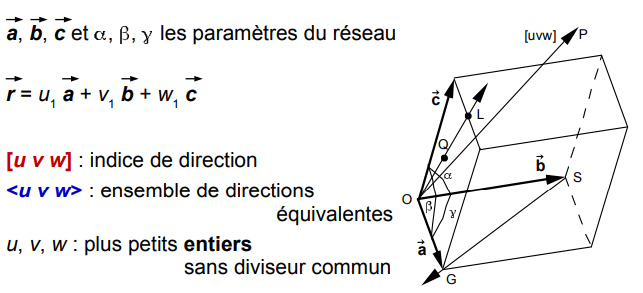
\includegraphics[scale = 0.5]{Miller_1.png}
        \item Notations des plans : Un plan cristallographique est décrit par $(hkl)$, où h,k, et l sont les indices de Miller représentant l'intersection du plan avec les axes du réseau. Les familles de plans équivalentes sont notées ${hkl}$. \\
        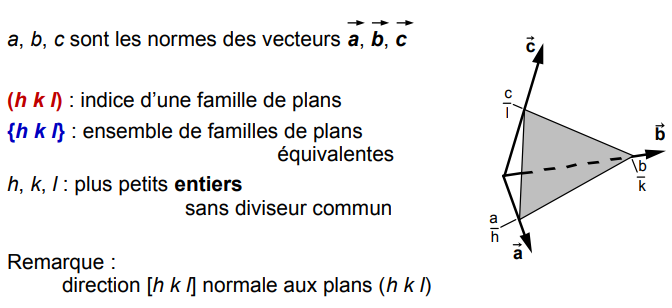
\includegraphics[scale = 0.5]{Miller_2.png}
    \end{itemize}
    \pagebreak
    \subsection{Défauts Cristallins}
    Les défauts dans les cristaux sont des perturbations dans l'ordre parfait des arrangements atomiques. Ils peuvent être classés en plusieurs catégories.
    
        \subsubsection{Défauts ponctuels (0D)}
        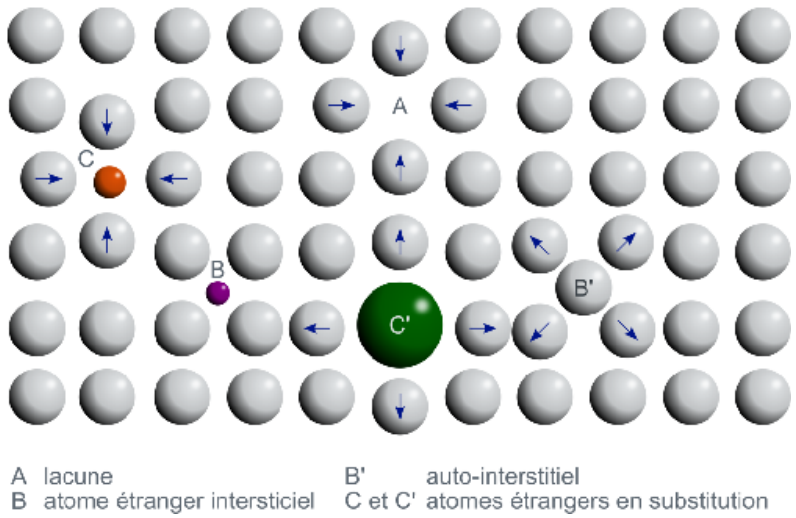
\includegraphics[scale = 0.3]{defauts_ponctuels.png}
        \begin{itemize}
            \item Lacunes : Absence d'un atome dans un site du réseau cristallin. 
            \item Atomes interstitiels : Atomes situés dans des positions interstitielles non occupées normalement. 
            \item Atomes de substitution : Atomes étrangers remplaçant les atomes du réseau.
        \end{itemize}
        
        \subsubsection{Défauts linéaires (1D)}
        \textbf{Dislocations} : Défauts liés au déplacement d'une partie du réseau. Il y a deux types principaux :
        \begin{itemize}
            \item Dislocation coin : Caractérisée par un vecteur de Burgers perpendiculaire à la ligne de dislocation.
            \item Dislocation vis : Caractérisée par un vecteur de Burgers parallèle à la ligne de dislocation.
        \end{itemize}
        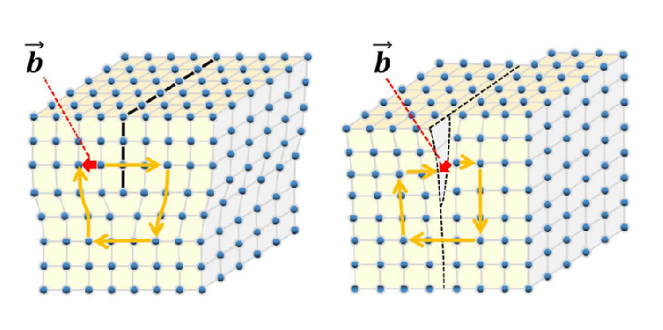
\includegraphics[scale=0.5]{dislocations_vis_et_coin.png}
        
        \subsubsection{Défauts bidimensionnels (2D)}
        \begin{itemize}
            \item Joints de grains : Interfaces entre des grains de différentes orientations.
            \item Macles : "Basculement" d’une partie du réseau par rapport à une autre. \\
            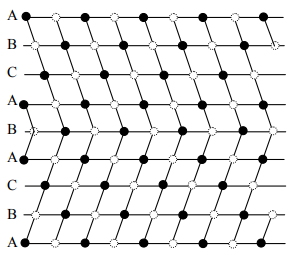
\includegraphics[scale=0.5]{macles.png}
            \item Défauts d'empilement : Perturbations dans l'ordre d'empilement des plans atomiques. \\
            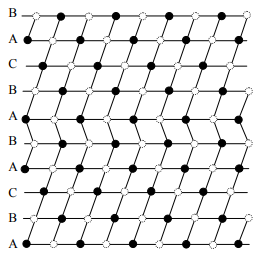
\includegraphics[scale=0.58]{defauts_d_empilement.png}
        \end{itemize}
        
        
        \subsubsection{Défauts tridimensionnels (3D)}
        \begin{itemize}
            \item Précipités : Zones de composition chimique différente au sein d'une matrice solide, pouvant être cohérentes ou incohérentes. \\
            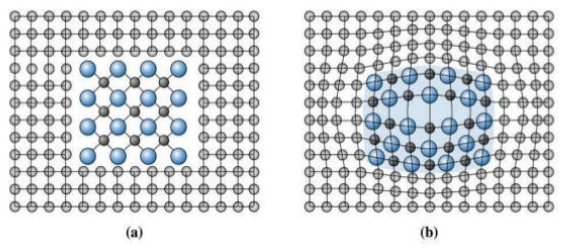
\includegraphics[width=1\linewidth]{Images/precipites.png}
        \end{itemize}
        \pagebreak
        \subsubsection{Phase amorphe}
        L'état amorphe d'un matériau se caractérise par un \textbf{désordre structurel} et l'\textbf{absence d'ordre à longue distance}, contrairement aux solides cristallins qui possèdent une structure régulière et périodique.
        \begin{itemize}
            \item Matériaux amorphes : Les matériaux tels que certains verres minéraux et polymères (thermoplastiques amorphes, thermodurs, élastomères) ne présentent pas d'ordre cristallin.
            \item Transition vitreuse : Lorsqu'un liquide se refroidit rapidement et n'a pas le temps de cristalliser, il se transforme en solide amorphe, ou "verre". La température de transition vitreuse $T_g$ est une mesure de cette transition. Elle dépend de la vitesse de refroidissement : une vitesse de refroidissement plus lente permet une réorganisation plus facile des atomes, abaissant ainsi $T_g$.
        \end{itemize}
    
    \subsection{Polymères}
        \subsubsection{Classification}
        Les polymères sont classés en fonction de leur comportement thermique et structure.
        
        \begin{itemize}
            \item Thermoplastiques amorphes : Ces polymères deviennent visqueux ou fondent à haute température et sont solubles dans certains solvants.\\ Exemples : polystyrène (PS), polyméthacrylate de méthyle (PMMA).
            \item Thermoplastiques semi-cristallins : Présentent à la fois des phases cristallines et amorphes. Ils ramollissent avant de fondre complètement.\\ Exemples : polyéthylène (PE), polypropylène (PP).
            \item Thermodurs : Polymères réticulés formant des réseaux tridimensionnels qui deviennent insolubles et infusibles après durcissement.\\ Exemples : résines époxy, bakélite.
            \item Élastomères : Polymères présentant une élasticité remarquable. Ils peuvent s'étirer et reprendre leur forme initiale après relâchement.\\ Exemples : caoutchouc naturel (polyisoprène), polybutadiène (PB).
        \end{itemize}
        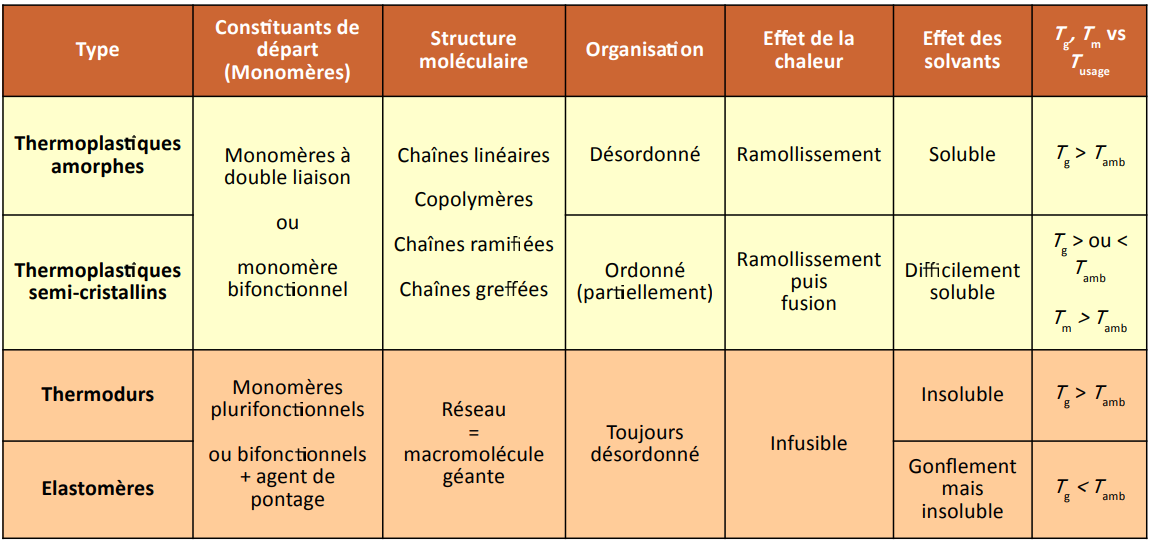
\includegraphics[width=1\linewidth]{Images/table_polymeres.png}
    
        \subsubsection{Structure}
        Les polymères peuvent avoir différentes structures moléculaires qui influencent leurs propriétés :
    
        \begin{itemize}
            \item Tacticité : La disposition des substituants le long de la chaîne polymérique peut être isotactique (ordonnée), syndiotactique (alternée), ou atactique (aléatoire), affectant ainsi la capacité du polymère à cristalliser.
            \begin{itemize}
                \item Isotactique : Tous les substituants se trouvent du même côté de la chaîne, permettant une cristallisation facile. \\
                    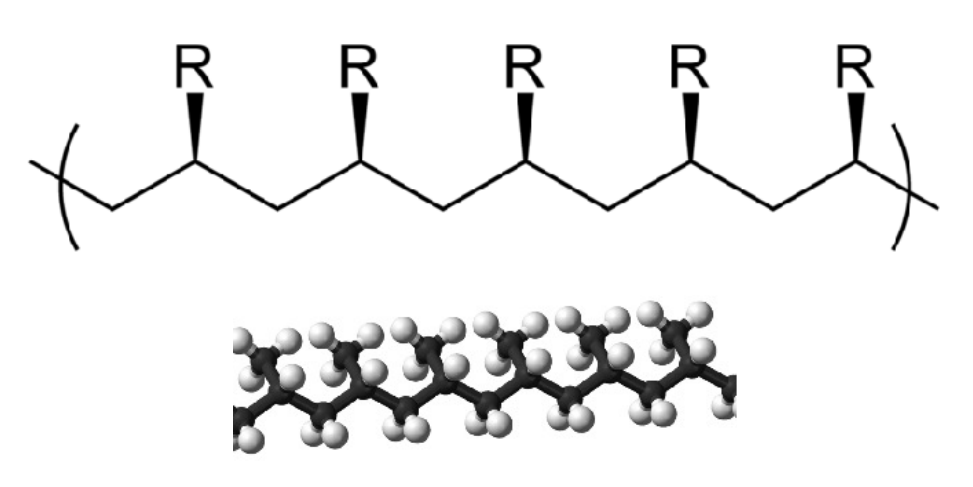
\includegraphics[width=0.6\linewidth]{Images/isotactique.png}
                \item Syndiotactique : Les substituants alternent de chaque côté, favorisant aussi la cristallisation. \\
                    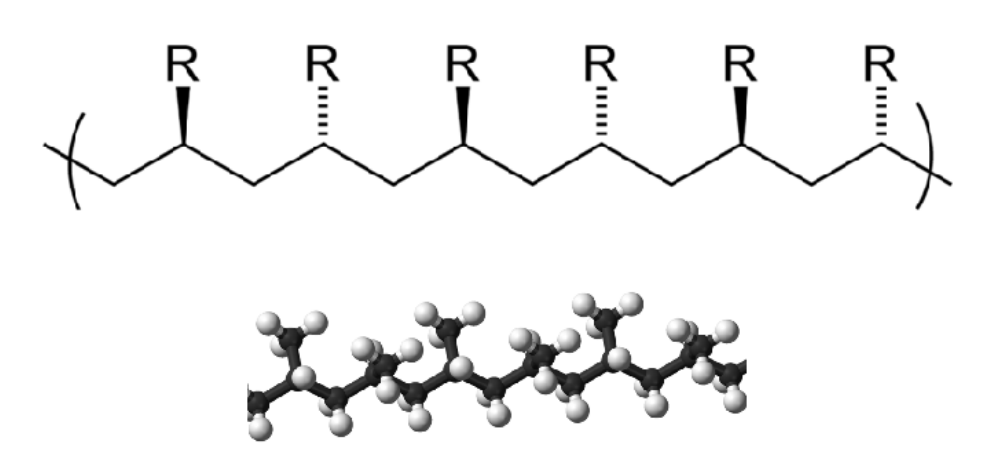
\includegraphics[width=0.6\linewidth]{Images/syndiotactique.png}
                    \pagebreak
                \item Atactique : Les substituants sont disposés aléatoirement, empêchant la cristallisation. \\
                    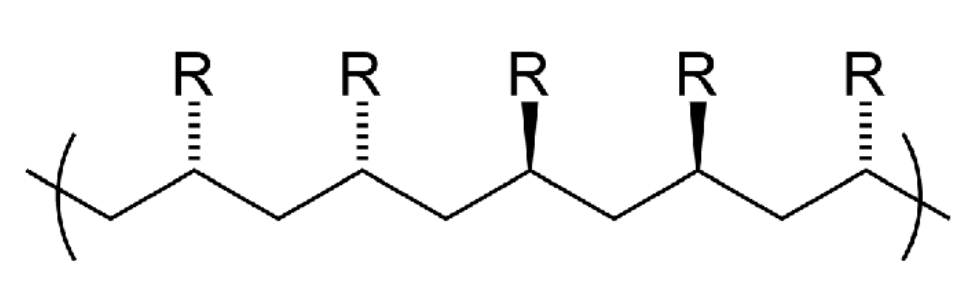
\includegraphics[width=0.6\linewidth]{Images/atactique.png}
            \end{itemize}
            \item Degré de polymérisation (DP) : Représente le nombre de monomères dans une chaîne polymérique. Un degré de polymérisation élevé conduit généralement à des propriétés mécaniques supérieures.
            \item Indice de polydispersité (PDI) : Indique la distribution de la masse moléculaire d'un polymère. Un PDI proche de 1 indique une distribution étroite, tandis qu'un PDI élevé indique une distribution large.
        \end{itemize}
    
        \subsubsection{Propriétés Thermiques}
        Les propriétés thermiques des polymères sont essentielles pour déterminer leur usage pratique :
        \begin{itemize}
            \item Température de transition vitreuse ($T_g$) : Température à laquelle un polymère amorphe passe d'un état vitreux rigide à un état caoutchoutique visqueux.
            \item Température de fusion ($T_m$) : Température à laquelle un polymère semi-cristallin fond. Les polymères amorphes n'ont pas de température de fusion définie.
        \end{itemize}
        Ces deux propriétés, ainsi que l'enthalpie de fusion et cristallisation peuvent être déterminées via une Calorimétrie différentielle à balayage (DSC en anglais). Elle permet aussi d'évaluer le taux de cristallinité d'un polymère, en se basant sur l'enthalpie de fusion.
    
        \subsubsection{Réactions de polymérisation}
        La formation de polymères se fait principalement par deux types de réactions de polymérisation :
        \begin{itemize}
            \item Polymérisation en chaîne : Implique la formation rapide de chaînes longues par addition de monomères à des sites actifs, tels que des radicaux libres, cations, anions, ou complexes de coordination. Exemples : polymérisation radicalaire de l'éthylène en polyéthylène.
            \item Polymérisation par étapes : Implique des réactions entre des monomères difonctionnels ou multifonctionnels pour former des polymères à travers des étapes successives de réaction. Exemples : formation de polyamides (nylon) et polyesters.
        \end{itemize}
    
        \subsubsection{Structure des polymères semi-cristallins}
        Les polymères semi-cristallins montrent une structure complexe due à la coexistence de régions amorphes et cristallines :
        \begin{itemize}
            \item Sphérolites : Structures sphériques formées par cristallisation des polymères semi-cristallins. Ils sont constitués de lamelles cristallines séparées par des régions amorphes. Les sphérolites influencent les propriétés mécaniques et optiques des polymères.
            \item Lamelles : Fines plaques cristallines au sein des sphérolites. La croissance et la taille des lamelles sont influencées par les conditions de cristallisation.
        \end{itemize}
\pagebreak
\section{Thermodynamique des matériaux et genèse des microstructures}
    \subsection{Thermodynamique des systèmes hétérogènes}
        \subsubsection{Règle des Phases de Gibbs}
        La règle des phases de Gibbs est une relation qui décrit le nombre de degrés de liberté ($F$) dans un système en équilibre thermodynamique. Elle est donnée par la formule :
        \begin{center}
            $F=C-P+2$
        \end{center}
        où :
        \begin{itemize}
            \item C est le nombre de constituants indépendants.
            \item P est le nombre de phases présentes.
        \end{itemize}
    
        \subsubsection{Coexistence de deux phases à l'équilibre}
        Lorsqu'il y a coexistence de deux phases (par exemple, liquide et vapeur, ou deux solides avec des structures cristallines différentes), l'équilibre thermodynamique est atteint lorsque les potentiels chimiques des composants sont égaux dans chaque phase. Cela se traduit par l'égalité des enthalpies libres molaires partielles entre les phases. La construction de la tangente commune aux courbes d'enthalpie libre molaire des deux phases permet de déterminer les compositions à l'équilibre et la proportion de chaque phase. \\
            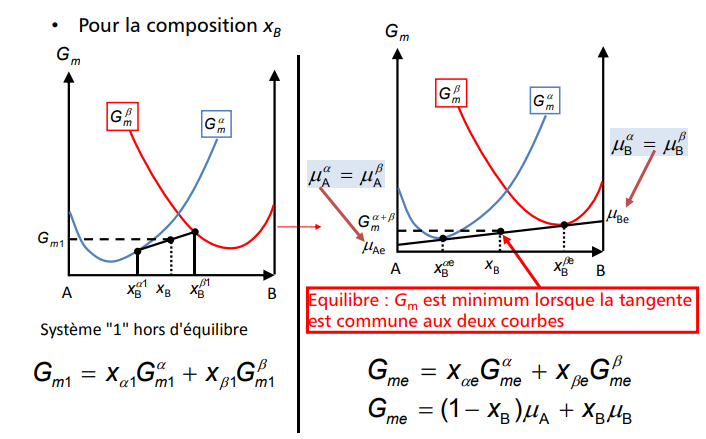
\includegraphics[width=.9\linewidth]{Images/phases_a_l_equilibre.png}
    
        \subsubsection{Systèmes à deux phases avec solubilité mutuelle complète}
        Dans un système binaire où les deux phases (solide et liquide) ont une solubilité mutuelle complète, les diagrammes de phase montrent des courbes "solidus" et "liquidus" définissant les limites de température entre les phases solides et liquides. En fonction de la température et de la composition, le système peut être entièrement liquide, entièrement solide, ou présenter une coexistence des deux phases. \\
            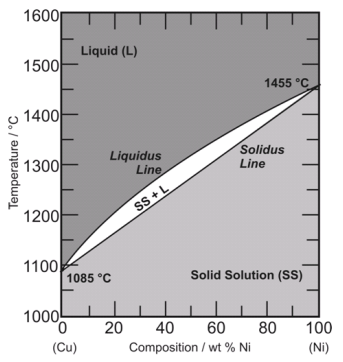
\includegraphics[width=0.5\linewidth]{Images/solubilite_mutuelle_complete.png}
    
        \subsubsection{Systèmes binaires endothermiques}
        Pour les systèmes binaires endothermiques, la dissolution d'un composant dans l'autre absorbe de la chaleur ($\Delta_{sol} H_m > 0$). Ces systèmes montrent une tendance à la séparation des composants à l'état solide, conduisant à la formation de deux phases solides distinctes à des compositions spécifiques. Dans les diagrammes de phase, cela se manifeste par des domaines biphasés, appellés "lacunes de solubilité". \\
            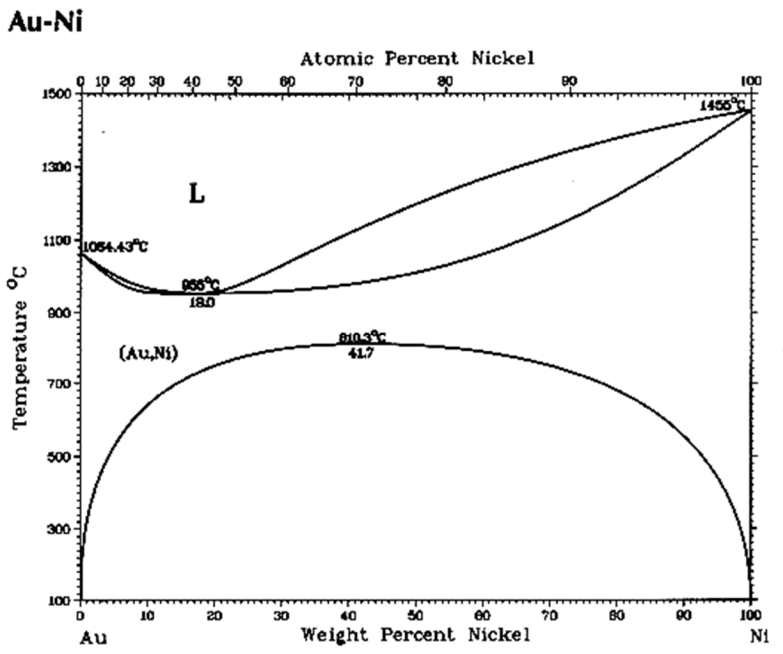
\includegraphics[width=.6\linewidth]{lacune_de_solubilite.png} \\
        \pagebreak \\
        Lorsque la lacune de solubilité (phase du bas sur le schéma ci-dessus) atteint la courbe du solidus, on a un \textbf{eutectique} : \\
            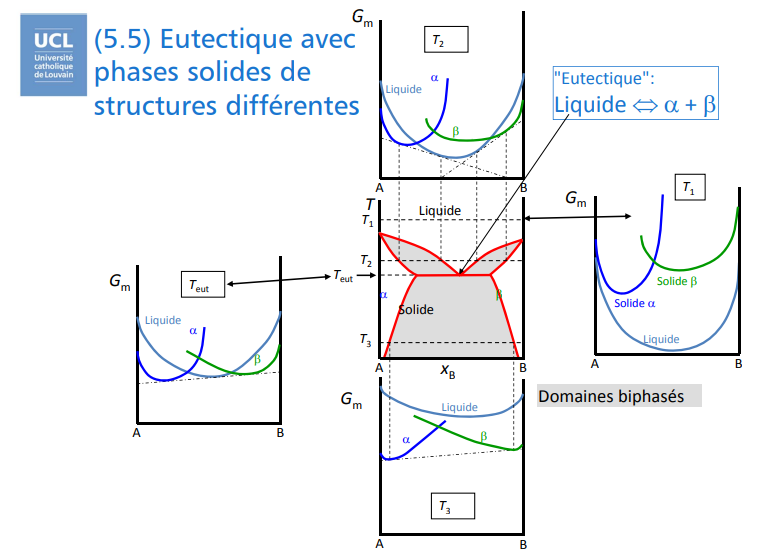
\includegraphics[width=.8\linewidth]{Images/eutectique.png} \\
        Lorsque les températures de fusion des 2 espèces sont fortement différentes, on peut voir apparaître une \textbf{péritectique} : \\
            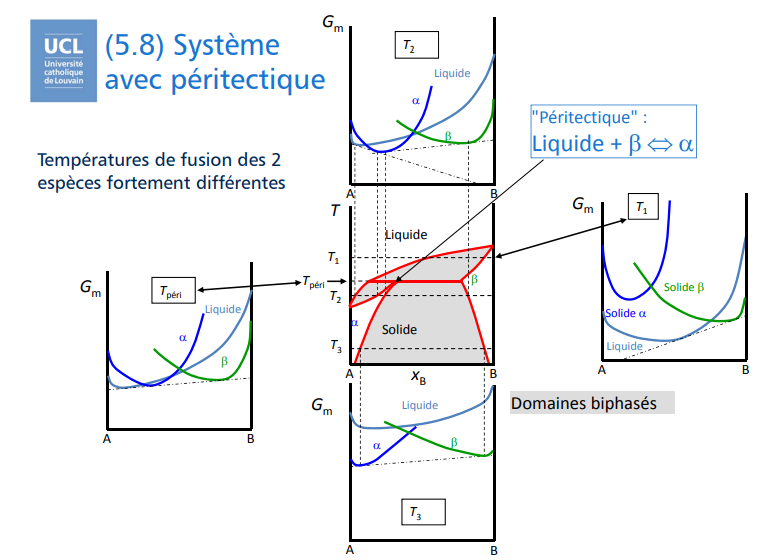
\includegraphics[width=0.8\linewidth]{Images/péritectique.png}
        \pagebreak \\
        \subsubsection{Systèmes binaires exothermiques}
        Les systèmes binaires exothermiques, où la dissolution libère de la chaleur ($\Delta_{sol} H_m<0$), montrent une tendance à la formation de phases ordonnées ou de composés intermédiaires. Dans ces systèmes, les interactions attractives entre différents composants favorisent la formation de structures ordonnées à l'état solide, ce qui peut soit être représenté par des courbes de phase montrant des minima distincts, soit la formation d'un composé intermédiaire. \\
            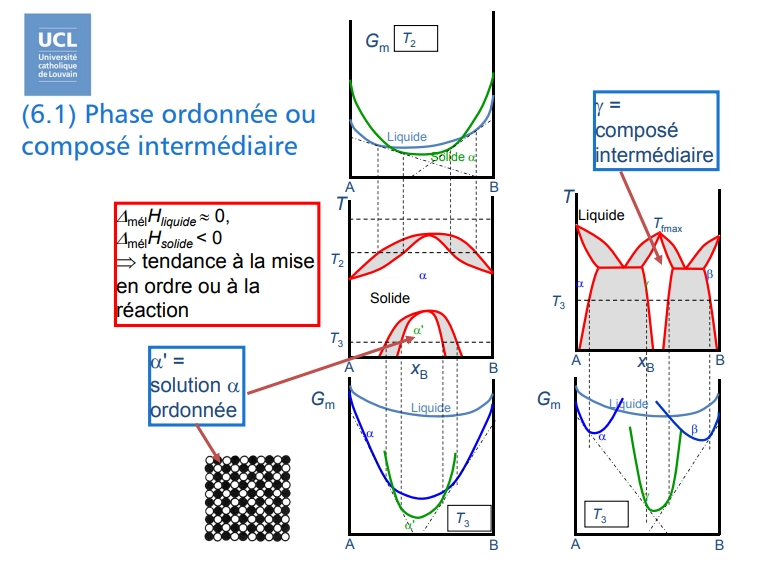
\includegraphics[width=0.8\linewidth]{sb_exothermique.png}
    
        \subsubsection{Couples de diffusion}
        Les couples de diffusion se forment lorsque deux phases solides pures sont mises en contact et qu'il y a diffusion de composants à travers l'interface. À l'équilibre, la composition des phases varie progressivement de l'une à l'autre, établissant des gradients de concentration et de potentiel chimique à travers l'interface. Ce processus est essentiel pour comprendre la formation de microstructures dans les alliages métalliques et les céramiques.

    \pagebreak
    \subsection{Thermodynamique des interfaces}
    La thermodynamique des interfaces traite des propriétés physiques et des équilibres thermodynamiques dans les régions où coexistent deux phases différentes. Elle couvre les concepts d'excès de grandeurs, d'énergie et de tension d'interface, ainsi que le mouillage et la forme des cristaux à l'équilibre.
        \subsubsection{Grandeurs d'excès et courbure}
        \begin{itemize}
            \item Interface : C'est une région où deux phases différentes coexistent, comme liquide/vapeur, solide/vapeur, ou solide/solide.
            \item Grandeurs d'excès : Dans le modèle de Gibbs, l'interface est représentée par une surface idéale. Les grandeurs comme le nombre de moles ($n_i$) sont ajustées pour respecter les bilans totaux des phases en définissant une grandeur d'excès ($n_i^s$) à l'interface. Cela dépend du plan de division choisi.
            \item Courbure de l'interface : La courbure d'une interface est définie par deux rayons principaux ($r_1$ et $r_2$), qui peuvent être positifs ou négatifs selon que l'interface est convexe ou concave par rapport à une phase.
        \end{itemize}

        \subsubsection{Énergie d'interface}
        \begin{itemize}
            \item Énergie d'interface ($\gamma$) : C'est l'énergie requise pour créer une unité de surface d'interface entre deux phases. À l'équilibre thermodynamique, les conditions incluent l'égalité des températures et des potentiels chimiques entre les phases ($T^\prime = T^{\prime\prime}$ et $\mu_i^\prime = \mu_i^{\prime\prime}$)
            \item Équation de Laplace: Cette équation relie la différence de pression entre deux côtés d'une interface courbe à la tension d'interface et aux rayons de courbure:
            \begin{center}
                $\Delta p = \gamma (\frac{1}{r_1}+\frac{1}{r_2})$
            \end{center}
        \end{itemize}

        \subsubsection{Tension d'interface}
        \begin{itemize}
            \item Tension d'interface ($\sigma$) : Elle est définie comme la force par unité de longueur exercée le long du périmètre de l'interface. Pour les interfaces fluides, la tension d'interface est équivalente à l'énergie d'interface ($\sigma = \gamma$).
            \item Mesure de la tension d'interface : Pour un film liquide, la tension d'interface peut être mesurée comme le travail nécessaire pour augmenter l'aire du film tout en maintenant les volumes des phases constantes.
        \end{itemize}
        \pagebreak
        
        \subsubsection{Mouillage}
        \begin{itemize}
            \item Ligne triple : C'est la ligne de rencontre de trois phases distinctes, par exemple, solide, liquide, et vapeur. À l'équilibre, les tensions d'interface le long de cette ligne doivent se compenser. \\
            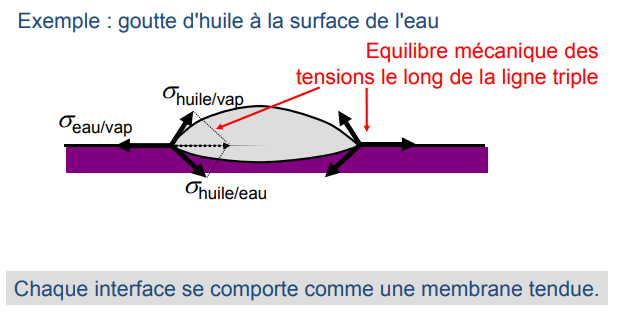
\includegraphics[width=.75\linewidth]{Images/ligne_triple.png}
            \item Angle de mouillage ($\theta$) : Définit l'étendue à laquelle un liquide mouille une surface solide. Il est lié aux tensions de surface par l'équation de Young :
            \begin{center}
                $\gamma_{sv} = \gamma_{sl} + \gamma_{lv} \: cos \: \theta$
            \end{center}
            Le mouillage complet se produit si $\theta = 0^\circ$ , et le non-mouillage se produit si $\theta = 180^\circ$. \\
                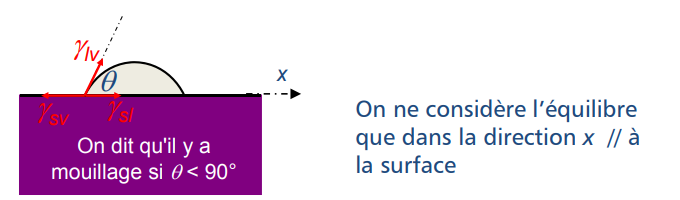
\includegraphics[width=0.75\linewidth]{Images/mouillage.png}
        \end{itemize}
        \pagebreak
        
        \subsubsection{Forme d'équilibre des cristaux}
        \begin{itemize}
            \item Anisotropie de l'énergie interfaciale : Dans les cristaux solides, l'énergie d'interface dépend de l'orientation cristallographique, ce qui signifie que certaines directions de croissance sont plus favorables que d'autres.
            \item Forme d'équilibre des cristaux : Dictée par la minimisation de l'énergie totale de surface, la forme à l'équilibre des précipités ou des cristaux est déterminée par les énergies relatives des différentes interfaces cristallines.
        \end{itemize}
            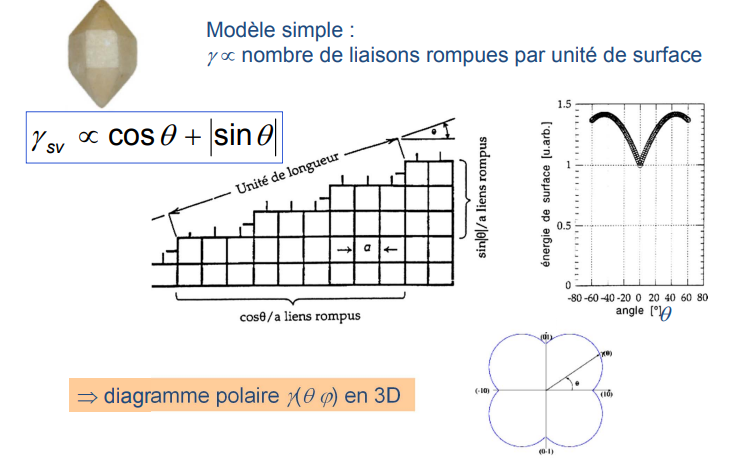
\includegraphics[width=0.75\linewidth]{Images/forme_d_equilibre_cristaux.png}
    \pagebreak
    
    \subsection{Transformation de phase}
    Les transformations de phase impliquent des changements dans les états des matériaux (ex. solidification, vaporisation) ou des modifications de la structure et des proportions des phases dans des systèmes multiphasés. Ces transformations sont guidées par des forces motrices et résistives qui déterminent la dynamique et la stabilité des nouvelles phases formées.

        \subsubsection{Forces motrices et résistives}
        \begin{itemize}
            \item Force motrice : La transformation de phase est principalement entraînée par une différence d'enthalpie libre ($\Delta G$) entre les états initial et final. Une transformation spontanée se produit lorsque $\Delta G < 0$, indiquant une enthalpie libre inférieure dans la nouvelle phase, ce qui constitue la force motrice de la transformation.
            \item  Forces résistives : Malgré une force motrice favorable, des barrières d'énergie (énergie d'activation $\Delta G^*$) doivent être surmontées pour que la transformation se produise. Ces barrières sont dues à la création d'interfaces et à d'autres résistances à la transition de phase. La probabilité de franchir ces barrières dépend de la température, comme décrit par la loi d'Arrhénius.
                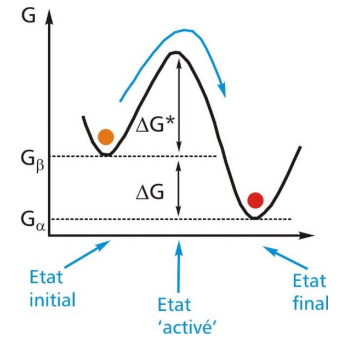
\includegraphics[width=0.5\linewidth]{Images/forces_motrices_et_resistives.png}
        \end{itemize}

        \subsubsection{Germination Homogène}
        La germination homogène se produit dans tout le volume du matériau sans préférence pour des sites spécifiques. Elle nécessite généralement une surfusion ou une surchauffe significative pour initier la transformation.
        \begin{itemize}
            \item Contribution volumique et interfaciale : La germination homogène implique deux contributions principales à l'enthalpie libre :
            \begin{itemize}
                \item Contribution volumique ($-V_s \Delta G_v$) : Gain d'énergie associé à la formation de la nouvelle phase.
                \item Contribution interfaciale ($A_{sl} \gamma_{sl}$) : Coût énergétique associé à la création d'une interface entre les phases initiale et nouvelle. \\
            \end{itemize}
                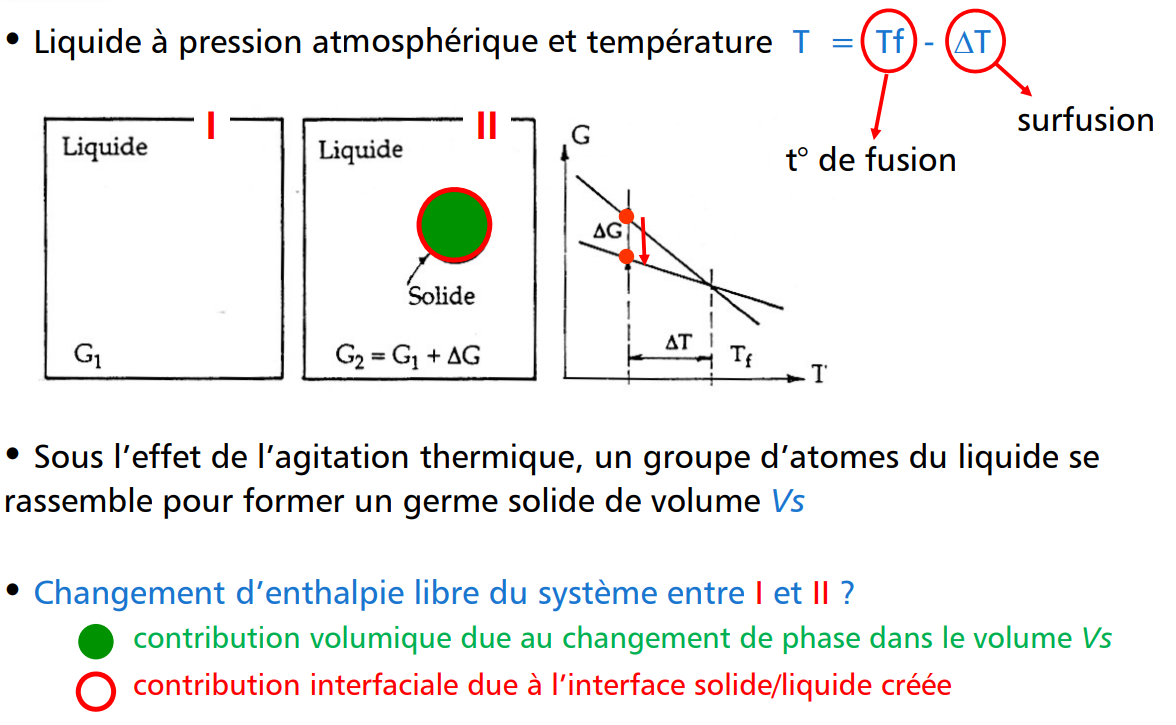
\includegraphics[width=0.75\linewidth]{Images/contribution_surfacique_et_volumique.png}
            \item Barrière de potentiel : La formation d'un germe stable nécessite de surmonter une barrière de potentiel. Le rayon critique ($r_c$) est la taille minimale que doit atteindre un germe pour que sa croissance réduise l'enthalpie libre du système. Pour un germe sphérique, $\Delta G = - V_s \Delta G_v + A_{sl} \gamma_{sl}$, où $\Delta G$ atteint un maximum à $r = r_c$. \\
                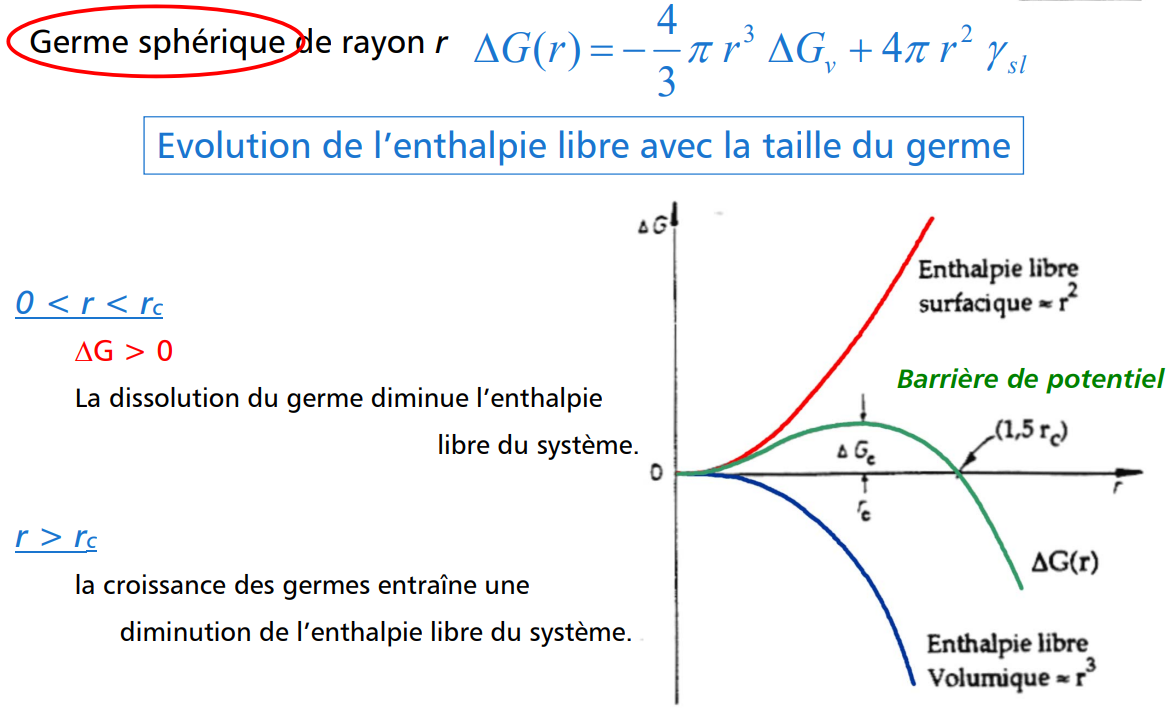
\includegraphics[width=0.75\linewidth]{Images/barriere_de_potentiel.png}
        \end{itemize}

        \subsubsection{Germination hétérogène}
        La germination hétérogène se produit sur des surfaces préexistantes (impuretés, interfaces, parois du récipient) qui réduisent la barrière énergétique pour la formation de germes.
        \begin{itemize}
            \item Avantage de la germination hétérogène : Elle nécessite une énergie d'activation ($\Delta G_c$) plus faible comparée à la germination homogène, car la présence de surfaces ou d'impuretés diminue l'énergie d'interface requise. La relation est donnée par :
            \begin{center}
                $\Delta G_{het} = S(\theta) \Delta G_{hom}$
            \end{center}
            où $S(\theta)$ est une fonction de l'angle de mouillage $\theta$. \\
                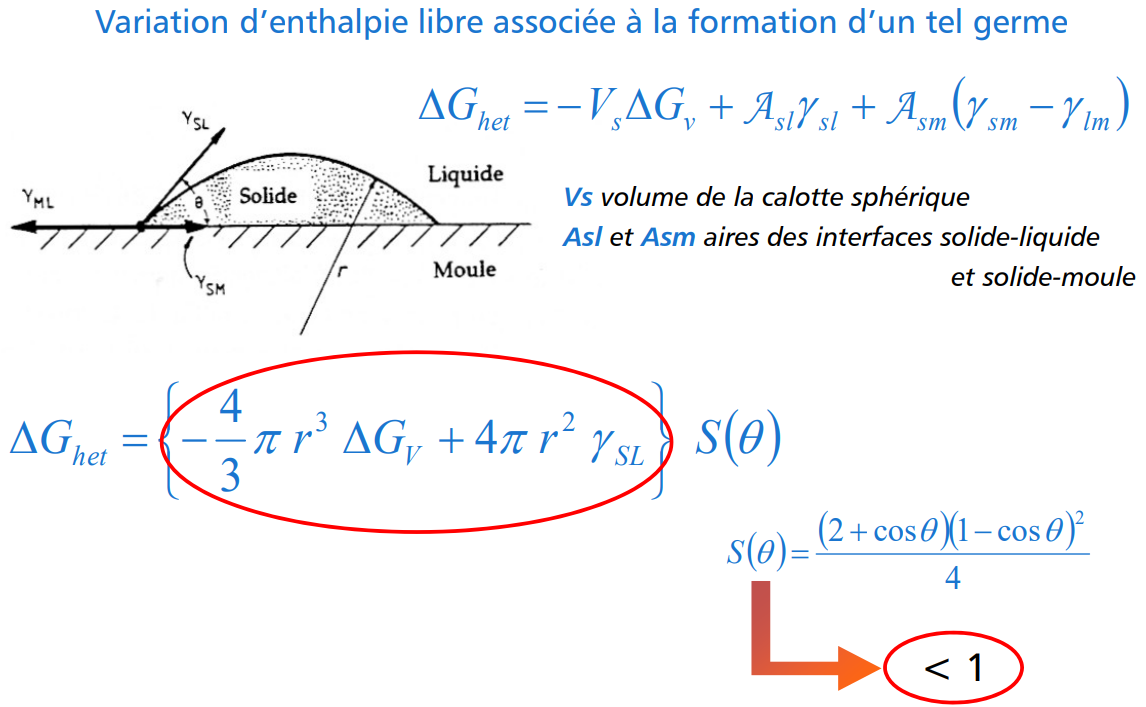
\includegraphics[width=0.75\linewidth]{Images/germination_heterogene.png}
            \item Exemples : La formation de brouillard ou de givre dans l'air où des particules de poussière servent de sites de germination pour les gouttelettes d'eau ou les cristaux de glace.
        \end{itemize}

        \subsubsection{Germination dans les phases non fluides}
        Contrairement aux liquides, les solides ont des propriétés spécifiques comme une énergie d'interface anisotrope et des contraintes locales dues aux différences de volume spécifique.
        \begin{itemize}
            \item Création d'un volume $V$ de la nouvelle phase $->$ Réduction de $-V \Delta G_v$
            \item Création d'une interface $\alpha / \beta$ d'aire $A_{\alpha \beta}$ $->$ Augmentation de $A_{\alpha \beta} \gamma_{\alpha \beta}$
            \item Différences dans les volumes spécifiques : Introduction de contraintes locales (énergie élastique) dues aux différences dans les volumes spécifiques des phases. \\
                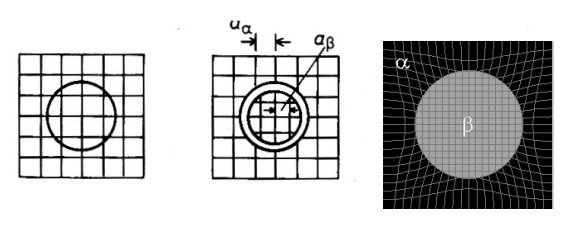
\includegraphics[width=0.5\linewidth]{Images/germination_phase_non_fluide.png}
        \end{itemize}
    \pagebreak

    \subsection{Diffusion}
    La diffusion est le processus par lequel les atomes ou les molécules se déplacent dans un matériau sous l'effet de gradients de concentration ou de potentiel chimique. Elle joue un rôle crucial dans de nombreux phénomènes de transformation de phase et dans l'établissement de l'équilibre dans les matériaux.

        \subsubsection{Introduction}
        Lorsqu'un système subit une transformation, par exemple une solidification ou une transformation de phase, la diffusion des éléments chimiques est souvent nécessaire pour atteindre l'équilibre. Par exemple, pendant la solidification, la composition du solide diffère de celle du liquide, nécessitant la diffusion pour ajuster les fractions volumiques et les compositions des phases. \\
            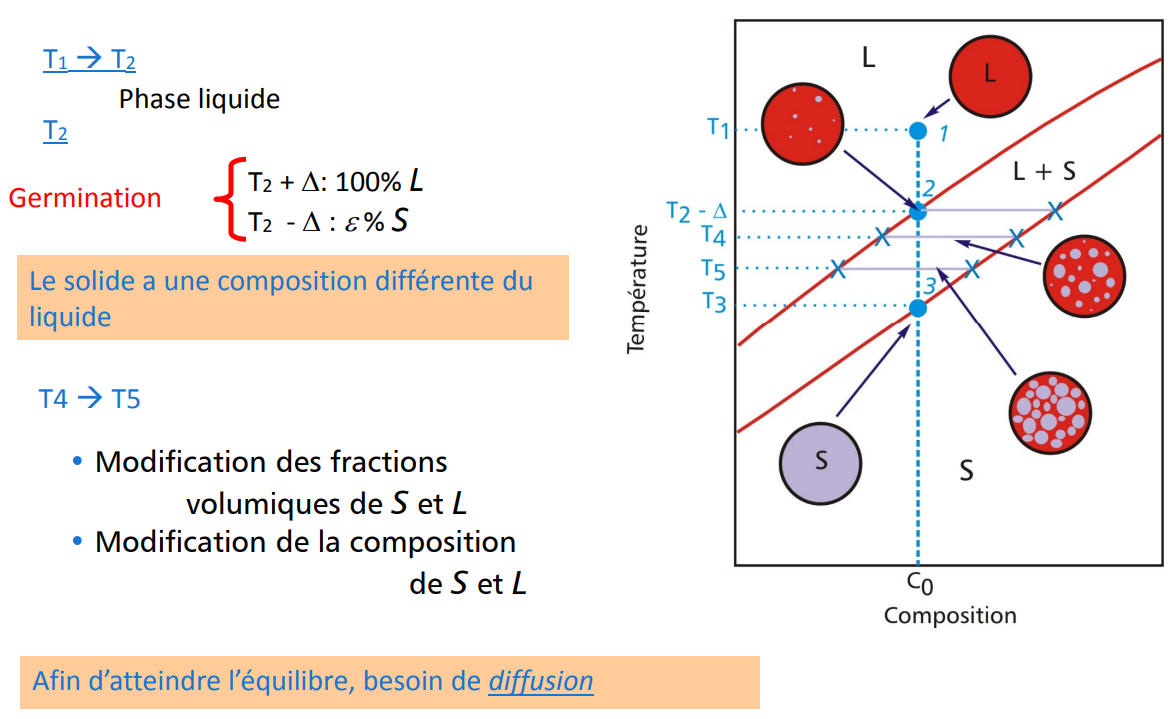
\includegraphics[width=0.75\linewidth]{Images/diffusion.png}

        \subsubsection{Transfert de matière et diffusion}
        \begin{itemize}
            \item Transfert de matière : Dans un système biphasé, le transfert de matière d'une phase à l'autre se produit spontanément si le potentiel chimique du constituant diminue lors du transfert.
            \item Gradient de potentiel chimique : La diffusion est principalement gouvernée par le gradient de potentiel chimique, qui peut correspondre ou être opposé au gradient de concentration.
            \item Diffusion vs convection : La diffusion est un flux de particules causé par des mouvements aléatoires dus à des gradients de potentiel chimique, tandis que la convection est le transport de matière par le mouvement global d'un fluide.
        \end{itemize}

        \subsubsection{Force motrice et flux de diffusion}
        \begin{itemize}
            \item Force motrice : Le gradient de potentiel chimique constitue la force motrice pour la diffusion.
            \item Flux de diffusion ($J$) : Il est défini comme le nombre d'atomes diffusant à travers une unité d'aire par unité de temps. Le flux est proportionnel au gradient de potentiel chimique ou de concentration :
            \begin{center}
                $J = -D \frac{\partial c}{\partial x}$
            \end{center}
            avec $D$ le coefficient de diffusion (voir la loi de Fick ci-dessous)
            \item Loi de Fick : La première loi de Fick décrit la diffusion sous un gradient de concentration, similaire à la loi de Fourier pour la conduction thermique.
                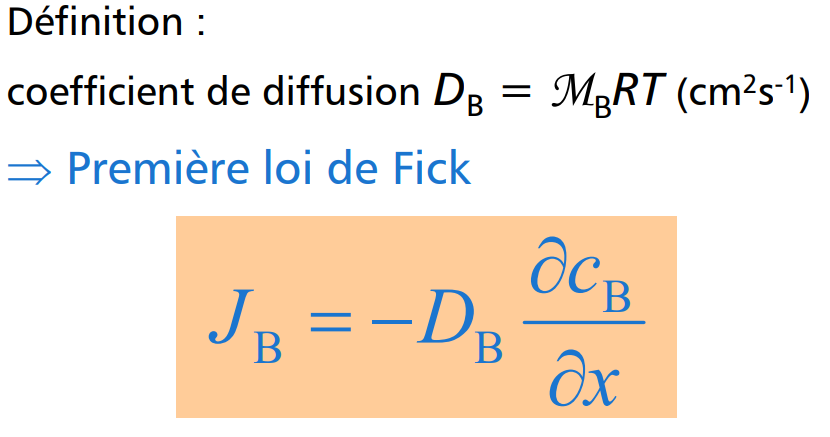
\includegraphics[width=0.75\linewidth]{Images/loi_de_fick.png}
        \end{itemize}

        \subsubsection{Mécanismes de diffusion à l'état solide}
        \begin{itemize}
            \item Mécanismes de diffusion :
            \begin{itemize}
                \item Diffusion interstitielle : Les atomes migrent à travers les sites interstitiels. Ce mécanisme est typiquement rapide.
                \item Diffusion par lacunes : Implique des échanges d'atomes avec des sites vacants ou lacunes dans le réseau cristallin. C'est un mécanisme plus lent car il dépend de la présence de lacunes.\\
                    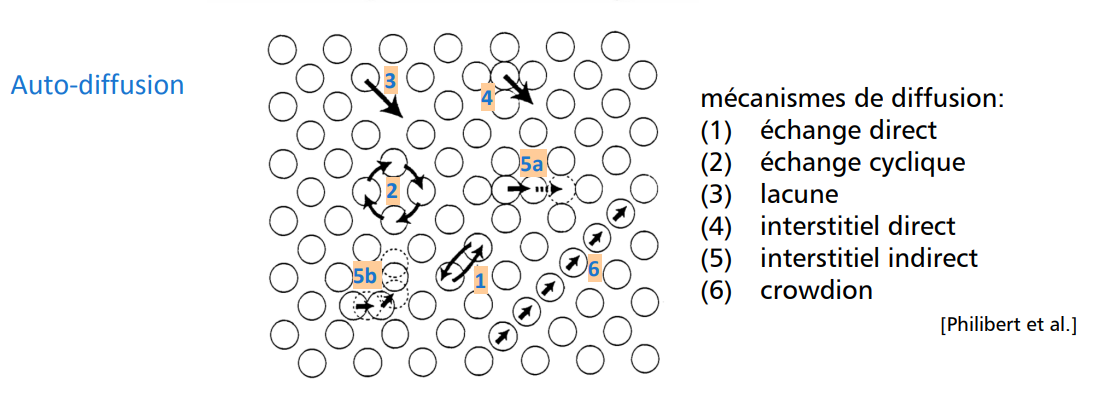
\includegraphics[width=0.9\linewidth]{Images/mecanismes_de_diffusion.png}
            \end{itemize}
            \item Saut aléatoire : Le modèle de saut aléatoire décrit le mouvement d'atomes entre des sites voisins, influencé par la fréquence de saut et la distance entre les sites.
            \pagebreak
            \item Coefficient de diffusion : Dépend de la fréquence de saut et de la distance de saut, variant selon la structure cristalline (cubic simple, centrée, ou à faces centrées). \\
                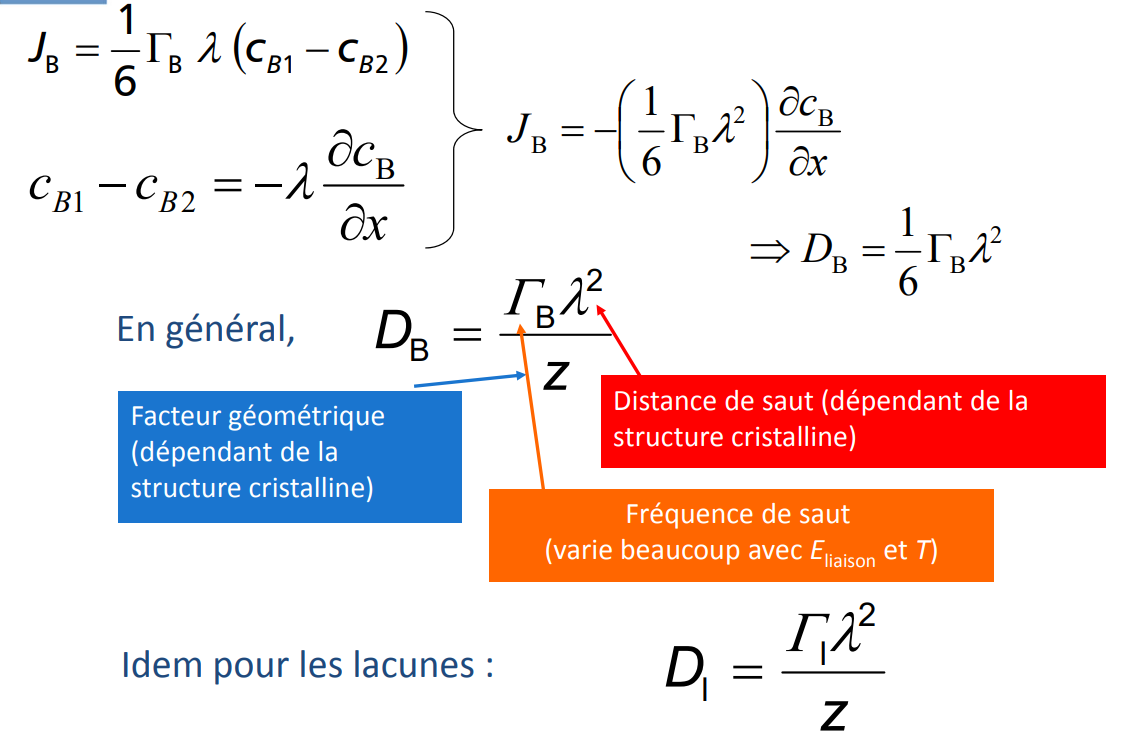
\includegraphics[width=0.75\linewidth]{Images/saut_aleatoire_et_lacunes.png} \\
                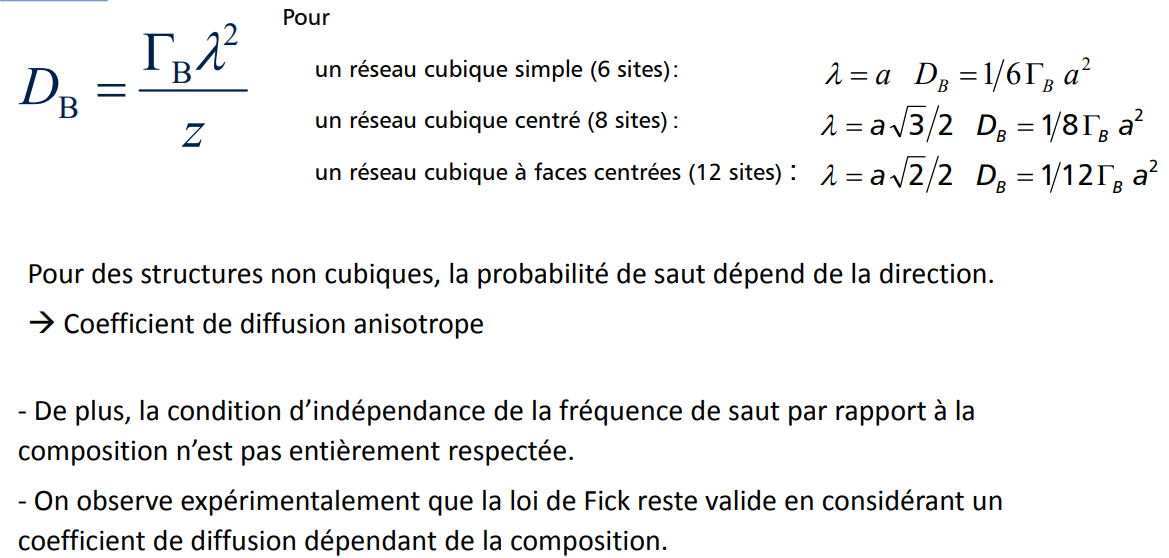
\includegraphics[width=0.75\linewidth]{Images/coefficient_diffusion.png}
        \end{itemize}

        \subsubsection{Influence de la température}
        Le coefficient de diffusion augmente exponentiellement avec la température, décrit par une relation d'Arrhenius :
        \begin{center}
            $D = D_0 exp(-\frac{\Delta H_{mig}}{RT})$
        \end{center}
        où $\Delta H_{mig}$ est l'enthalpie d'activation de la migration et $R$ est la constante des gaz parfaits.

        \begin{itemize}
            \item Énergie d'activation : Correspond à l'énergie nécessaire pour qu'un atome surmonte la barrière d'énergie et diffuse. Elle est généralement proportionnelle à la température de fusion du matériau.
            \item Diagramme d'Arrhenius : Utilisé pour représenter la variation logarithmique du coefficient de diffusion en fonction de l'inverse de la température. Les pentes sur ces diagrammes peuvent révéler des mécanismes de diffusion différents ou des courants de diffusion.
        \end{itemize}

\section{Électrons et Phonons}
    \subsection{Rappels de physique quantique}
    \begin{itemize}
        \item Mécanique quantique : Une discipline qui étudie les propriétés des particules à l'échelle atomique et subatomique. Elle introduit des concepts comme la dualité onde-corpuscule et la quantification de l'énergie.
        \item Équation de Schrödinger : Fournit une description mathématique de l'évolution des fonctions d'onde des particules. Les solutions de cette équation permettent de déterminer les niveaux d'énergie permis pour les électrons dans un atome ou un solide.
        \item Principe d'incertitude d'Heisenberg : Il est impossible de connaître simultanément et précisément la position et la quantité de mouvement d'une particule. Cela a des implications importantes sur le comportement des électrons dans les atomes et les solides.
        \item Principe d'exclusion de Pauli : Deux fermions (comme les électrons) ne peuvent occuper le même état quantique simultanément. Ceci explique la structure des niveaux d'énergie dans les atomes et les bandes d'énergie dans les solides.
    \end{itemize}

    \subsection{Le réseau réciproque}
    Le réseau réciproque est une construction mathématique utilisée pour décrire les propriétés périodiques d'un cristal. Chaque point du réseau réciproque correspond à une onde plane qui possède la même périodicité que le réseau direct du cristal.
    \begin{itemize}
        \item Utilisation : Le réseau réciproque est essentiel pour comprendre la diffraction des électrons et des rayons X dans les cristaux, ainsi que pour analyser les bandes d'énergie des électrons dans les solides.
        \item Propriétés : Le réseau réciproque d'un réseau cristallin présente les mêmes symétries que le réseau direct. Par exemple, le réseau réciproque d'un réseau cubique à faces centrées (CFC) est un réseau cubique centré (CC), et vice versa. (Matière hors cours)
    \end{itemize}

    \subsection{Modèle des électrons libres et quasi-libres dans les solides}
    Considère les électrons de valence dans un métal comme un gaz d'électrons libres qui se déplacent dans un potentiel constant créé par les ions du réseau. Ce modèle explique la conductivité électrique élevée des métaux.

    \begin{itemize}
        \item Gaz d'électrons dans un métal normal : Les électrons de valence se délocalisent et peuvent se déplacer librement dans tout le solide, formant un "gaz d'électrons". Ce comportement conduit à des propriétés de conduction électrique et thermique spécifiques.
        \item Modèle des électrons quasi-libres : Prend en compte l'effet du potentiel périodique du réseau cristallin sur les électrons libres. Ce modèle conduit à la formation de bandes d'énergie permises et interdites, déterminant si un matériau est un métal, un isolant ou un semi-conducteur.
        \item Théorie des bandes d'énergie : Explique la structure électronique des solides en termes de bandes d'énergie permises séparées par des bandes interdites. La position de l'énergie de Fermi par rapport aux bandes permet de déterminer les propriétés électroniques du matériau.
    \end{itemize}

    \subsection{Notion de "Phonon"}
    Dans un solide, les atomes vibrent autour de leurs positions d'équilibre. Ces vibrations peuvent être décrites comme des ondes élastiques progressives qui se propagent à travers le matériau.

    \begin{itemize}
        \item Phonons : Quasi-particules associées aux vibrations du réseau cristallin. Les phonons jouent un rôle clé dans les propriétés thermiques des solides, telles que la conductivité thermique.
        \item Modes de vibration : Incluent les ondes longitudinales et transversales. Le nombre total de modes de vibration est déterminé par le nombre d'atomes dans la maille cristalline et le type de réseau.
        \item Température de Debye : Une mesure de la limite supérieure des fréquences de vibration des phonons dans un solide. Elle est liée à la rigidité du solide et à sa densité.
    \end{itemize}
    
    \subsection{Chaleur spécifique dans les solides}
    La chaleur spécifique d'un solide est la quantité d'énergie requise pour augmenter la température d'une unité de masse d'une substance d'un degré Kelvin.

    \begin{itemize}
        \item Contributions à la chaleur spécifique :
        \begin{itemize}
            \item Chaleur spécifique électronique : Relativement faible par rapport à la chaleur spécifique du réseau, car seuls les électrons proches du niveau de Fermi contribuent à la chaleur spécifique.
            \item Chaleur spécifique du réseau : Dépend des vibrations des atomes dans le réseau cristallin (phonons). À basse température, elle suit une loi de puissance en $T^3$(loi de Debye), et à haute température, elle tend vers une constante (loi de Dulong et Petit).
        \end{itemize}
        \item Influence de la température : À très basse température, la chaleur spécifique est dominée par les contributions quantiques (oscillations de point zéro). À température ambiante, la chaleur spécifique du réseau est prédominante.
    \end{itemize}

\section{Conductivité Électrique}
    \subsection{Phénomènes de transport de charge}
    \begin{itemize}
        \item Phénomènes de transport : Concernent le mouvement de particules chargées (électrons, trous) ou non chargées (phonons) sous l'influence de forces extérieures comme un champ électrique, un gradient de température, ou un champ magnétique.
        \item Types de transport : Incluent le transport de charge (courant électrique) et le transport d'énergie (courant thermique). Les collisions entre particules, qu'elles soient avec d'autres particules ou des impuretés dans le matériau, tendent à ramener le système à l'équilibre.
    \end{itemize}

    \subsection{Conductivité électrique dans les métaux}
    \begin{itemize}
        \item Conductivité électrique ($\sigma$) : Mesure de la capacité d'un matériau à permettre le passage d'un courant électrique. Elle est inversement proportionnelle à la résistivité ($\rho$).
        \item Modèle classique : Les électrons se déplacent de manière diffusée dans le métal, subissant des collisions avec les ions du réseau cristallin et des impuretés.
        \item Approche quantique : Prend en compte la nature ondulatoire des électrons et la distribution de Fermi. Les électrons près de la surface de Fermi sont les principaux contributeurs à la conduction électrique.
    \end{itemize}

    \subsection{Mesure de Résistivité Électrique}
    \begin{itemize}
        \item Résistivité idéale ($\rho_i$) : Dépend des vibrations thermiques du réseau cristallin et augmente avec la température.
        \item Résistivité résiduelle ($\rho_r$) : Dépend des imperfections statiques du réseau (impuretés, lacunes). Elle est indépendante de la température.
        \item Loi de Matthiessen : La résistivité totale ($\rho$) d'un métal est la somme de $\rho_i$ et $\rho_r$. Cette loi explique la variation de résistivité en fonction de la température.
            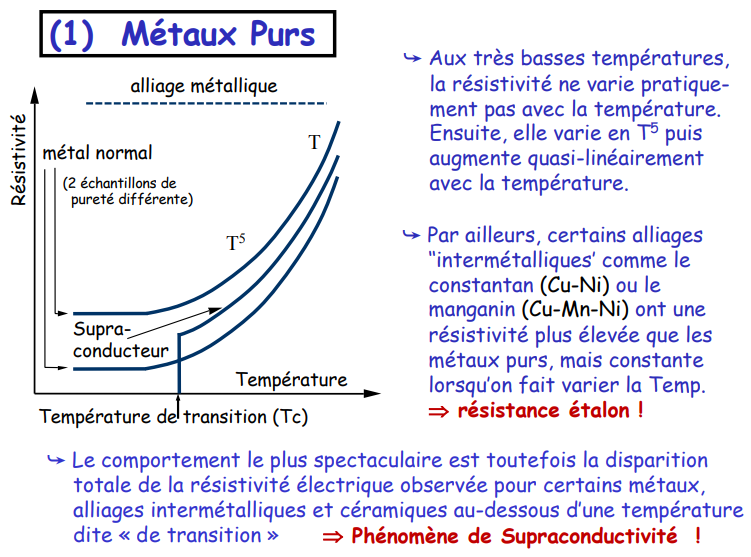
\includegraphics[width=0.75\linewidth]{Images/resistivites_electriques.png}
    \end{itemize}

    \subsection{Conductivité électrique (intrinsèque et extrinsèque) dans les semi-conducteurs purs et dopés}
    \begin{itemize}
        \item Semi-conducteurs intrinsèques : Matériaux purs où la conduction électrique est due à l'excitation thermique d'électrons de la bande de valence vers la bande de conduction.
        \item Semi-conducteurs extrinsèques : Dopage avec des impuretés donneuses (type n) ou accepteurs (type p) augmentant la conductivité. La densité de porteurs de charge (électrons et trous) dépend de la température et de la concentration en impuretés.
        \item Mobilité des porteurs de charge : Elle est influencée par les interactions avec le réseau et les impuretés, et varie inversement avec la température.
        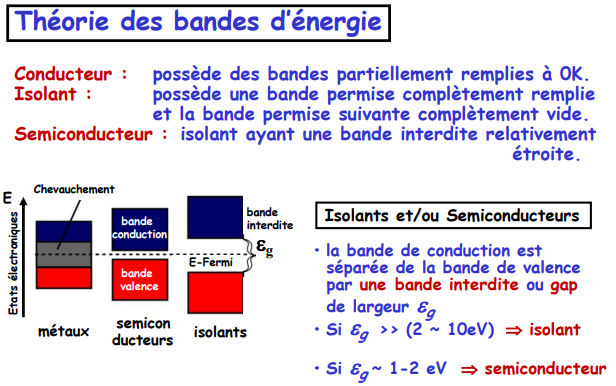
\includegraphics[width=0.75\linewidth]{Images/conductivite_bandes_energies.png}
    \end{itemize}

    \subsection{Introduction à la supraconductivité}
    Supraconductivité : Phénomène où certains matériaux présentent une résistance électrique nulle en dessous d'une température critique ($T_c$), observée pour la première fois dans le mercure à 4,2 K par Kamerlingh Onnes en 1911.

    \subsection{Effet Meisner, théorie BCS et applications}
    \begin{itemize}
        \item Effet Meissner : Phénomène par lequel un supraconducteur expulse tout champ magnétique interne lorsqu'il passe à l'état supraconducteur. Ceci rend le matériau parfaitement diamagnétique.
        \item Théorie BCS : Développée par Bardeen, Cooper, et Schrieffer, elle explique la supraconductivité par la formation de paires d'électrons (paires de Cooper) couplées à travers des vibrations du réseau cristallin (phonons).
        \item Applications : Utilisation des matériaux supraconducteurs dans des aimants pour les trains à lévitation magnétique (Maglev), l'imagerie par résonance magnétique (IRM), et les accélérateurs de particules. \\
            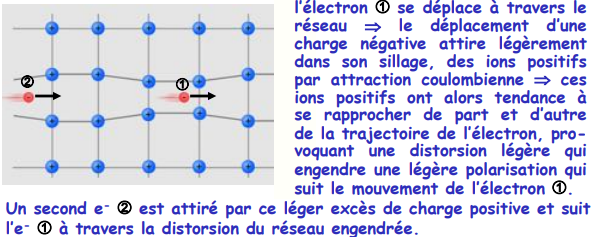
\includegraphics[width=0.75\linewidth]{Images/theorie_bcs.png}
    \end{itemize}

\section{Conductivité thermique}
    \subsection{Introduction au phénomène de transport d'énergie}
    Transport d'énergie : Lorsque différentes régions d'un système sont à des températures différentes, l'énergie thermique (chaleur) se transfère des régions les plus chaudes vers les plus froides. \\
    Mécanismes de transport : 
    \begin{itemize}
        \item Rayonnement (radiation) : Transfert de chaleur sous forme de rayonnement électromagnétique, plus intense à des températures élevées.
        \item Convection : Transfert de chaleur par le mouvement de portions d'un fluide. Cela implique l'échange de chaleur entre une surface et un fluide mobile en contact avec elle, causé par un gradient de température.
        \item Conduction : Transfert de chaleur à travers une substance solide, caractérisé par la transmission de l'agitation thermique des particules de proche en proche.
    \end{itemize}

    \subsection{Conductivité thermique électronique (loi de Wiedemann - Franz)}
    \begin{itemize}
        \item Conductivité thermique électronique ($k_E$) : Relie la capacité d'un matériau à conduire la chaleur par le mouvement des électrons. Dans les métaux, les électrons libres sont les principaux porteurs de chaleur.
        \item Loi de Wiedemann-Franz : Établit que la conductivité thermique électronique est proportionnelle à la conductivité électrique () d'un métal :
        \begin{center}
            $\frac{k_E}{\sigma T} = L$
        \end{center}
        où $L$ est le nombre de Lorentz (environ $2.45 \times 10^{-8} W \Omega K^{-2}$). \\
            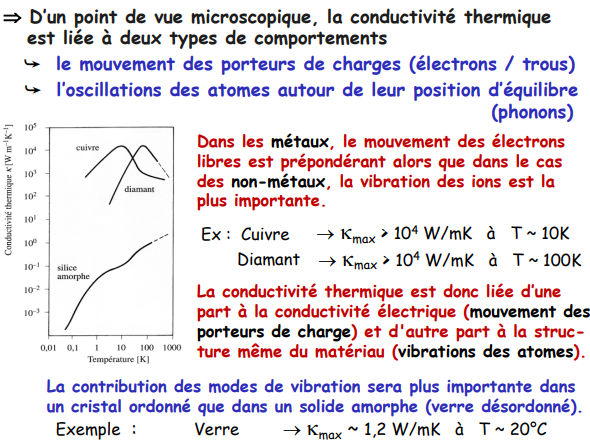
\includegraphics[width=0.75\linewidth]{Images/conduction_thermique_metaux_et_non_metaux.png}
    \end{itemize}

    \subsection{Conductivité thermique de réseau}
    La conductivité thermique de réseau ($k_g$) est due aux vibrations du réseau cristallin (phonons). Ce mécanisme est prédominant dans les isolants électriques où il n'y a pas d'électrons libres pour transporter la chaleur.
    \begin{itemize}
        \item Mécanismes de transport : La chaleur est transportée par des vibrations des atomes autour de leur position d'équilibre. Ces vibrations se propagent sous forme d'ondes (phonons) qui transportent l'énergie thermique du côté chaud au côté froid du cristal.
        \item Phonons et conductivité thermique :
        \begin{itemize}
            \item À basse température, la conductivité thermique augmente proportionnellement à $T^3$ (régime de Debye).
            \item À haute température, la conductivité thermique diminue en raison des interactions phonon-phonon, particulièrement des processus "umklapp" qui inversent la direction du flux de chaleur.
        \end{itemize}
            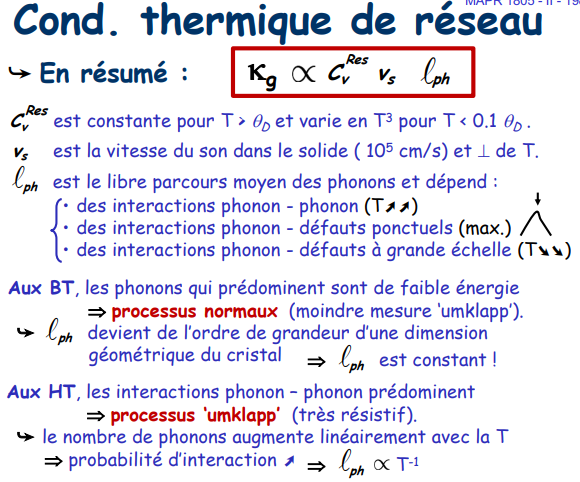
\includegraphics[width=0.75\linewidth]{Images/cond_thermique_reseau.png}
    \end{itemize}

\section{Propriétés diélectriques}
    \subsection{Description Électrostatique de la Matière (Matière Polarisée)}
    \begin{itemize}
        \item \textbf{Matière polarisée} : La matière est constituée de nombreuses charges électriques positives (noyaux atomiques) et négatives (électrons). En général, ces charges sont équilibrées, rendant la matière électriquement neutre.
        \item \textbf{Effet d'un champ électrique} : Lorsqu'un champ électrique externe est appliqué, les charges positives et négatives sont déplacées, créant une séparation des barycentres des charges positives et négatives. Cela induit une polarisation du matériau.
        \item \textbf{Polarisation} : Le vecteur polarisation ($P$) est défini comme le moment dipolaire par unité de volume. Pour un matériau homogène, isotrope, et linéaire, $P$ est proportionnel au champ électrique appliqué ($E$), caractérisé par la susceptibilité diélectrique ($\chi_e$) :
        \[
        P = \epsilon_0 \chi_e E
        \]
        où $\epsilon_0$ est la permittivité du vide.
    \end{itemize}
    
    \subsection{Notions de Dipôle Électrique Élémentaire et de Polarisation}
    
    \begin{itemize}
        \item \textbf{Dipôle électrique élémentaire} : Un dipôle est constitué de deux charges de magnitudes égales mais de signes opposés, séparées par une distance $d$. Le moment dipolaire ($p$) est donné par :
        \[
        p = Q \cdot d
        \]
        où $Q$ est la charge de chaque pôle du dipôle.
        \item \textbf{Polarisation} : Dans un matériau polarisé, un grand nombre de dipôles électriques sont alignés dans la direction du champ électrique appliqué. La polarisation totale d'un matériau est la somme vectorielle des moments dipolaires individuels par unité de volume.
        \item \textbf{Types de polarisation} : Incluent la polarisation électronique, ionique, d'orientation et d'interface, chacune contribuant différemment selon le type de matériau et les conditions extérieures.
    \end{itemize}
    
    \subsection{Principaux Mécanismes de Polarisation}
    
    \begin{itemize}
        \item \textbf{Polarisation électronique} : Déplacement des nuages électroniques par rapport aux noyaux atomiques sous l'influence d'un champ électrique. Ce type de polarisation est présent dans tous les matériaux et reste actif jusqu'à des fréquences très élevées (visible).
        \item \textbf{Polarisation ionique} : Déplacement relatif des ions positifs et négatifs dans un solide ionique (comme NaCl) sous l'effet d'un champ électrique. Ce mécanisme est particulièrement important dans les cristaux ioniques.
        \item \textbf{Polarisation d'orientation} : Concernant les molécules polaires, où les moments dipolaires permanents sont alignés par un champ électrique appliqué, ce qui est contrebalancé par l'entropie. Important dans les matériaux macroscopiques avec des molécules polaires, comme l'eau.
        \item \textbf{Polarisation d'interface} : Se produit dans les matériaux composites avec des régions conductrices entourées d'une matrice isolante. Les charges mobiles se déplacent dans les régions conductrices et s'accumulent aux interfaces, créant une distribution dipolaire macroscopique.
    \end{itemize}
    
    \subsection{Ferroélectricité, Piézoélectricité, Pyroélectricité, ...}
    
    \begin{itemize}
        \item \textbf{Ferroélectricité} : Propriété de certains matériaux qui présentent une polarisation électrique spontanée réversible par l'application d'un champ électrique externe. Les matériaux ferroélectriques ont une température critique, appelée température de Curie ($T_c$), en dessous de laquelle ils montrent une polarisation spontanée.
        \begin{itemize}
            \item \textit{Exemple} : Le titanate de baryum (BaTiO$_3$), qui passe par plusieurs transitions de phase structurales, montrant une polarisation dans différentes directions à différentes températures.
        \end{itemize}
        \item \textbf{Piézoélectricité} : Capacité de certains matériaux à générer une charge électrique en réponse à une contrainte mécanique. Tous les matériaux ferroélectriques sont aussi piézoélectriques, mais tous les piézoélectriques ne sont pas ferroélectriques.
        \begin{itemize}
            \item \textit{Application} : Utilisation dans les capteurs, les actionneurs, et les dispositifs médicaux.
        \end{itemize}
        \item \textbf{Pyroélectricité} : Propriété des matériaux à produire une charge électrique lorsqu'ils sont chauffés ou refroidis. Un cristal pyroélectrique possède une polarisation spontanée qui varie avec la température, sans nécessiter de champ électrique externe.
        \begin{itemize}
            \item \textit{Exemple} : Le quartz et les cristaux de wurtzite.
        \end{itemize}
        \item \textbf{Relation entre ces propriétés} :
        \begin{itemize}
            \item Un matériau pyroélectrique est nécessairement piézoélectrique, mais l'inverse n'est pas vrai.
            \item Les ferroélectriques, sous leur température critique, appartiennent à la classe des matériaux pyroélectriques car ils présentent une polarisation spontanée.
        \end{itemize}
            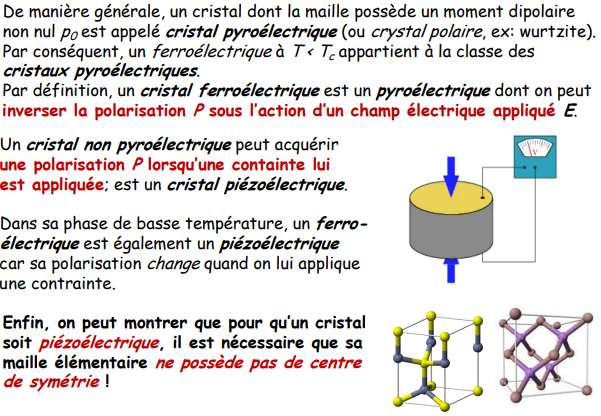
\includegraphics[width=0.75\linewidth]{Images/pyro_et_piezoelectricite.png}
    \end{itemize}

\section{Propriétés Magnétiques}
    \subsection{Description électromagnétique de la matière (matière aimantée)}
    \begin{itemize}
        \item \textbf{Matière aimantée} : Chaque atome (ou ion) d'un matériau possède un moment magnétique. Un matériau est dit aimanté si la somme vectorielle des moments magnétiques des atomes est non nulle.
        \item \textbf{Aimantation} : Le vecteur aimantation (\(M\)) est défini comme le moment magnétique par unité de volume. 
        \item \textbf{Induction magnétique} : Lorsqu'un matériau est placé dans un champ magnétique externe (\(B_c\)), il acquiert une aimantation \(M\). L'induction magnétique totale \(B\) est donnée par \(B = \mu_0 (H + M)\), où \(H\) est le champ magnétique externe et \(\mu_0\) la perméabilité du vide.
    \end{itemize}
    
    \subsection{Notions de dipôle magnétique élémentaire et d’aimantation}
    \begin{itemize}
        \item \textbf{Dipôle magnétique élémentaire} : Un dipôle magnétique est associé à une boucle de courant, telle qu'un électron en mouvement orbital ou un moment de spin. Le moment magnétique (\(m\)) d'un dipôle est donné par \(m = I A\), où \(I\) est l'intensité du courant et \(A\) l'aire de la boucle.
        \item \textbf{Aimantation} : L'aimantation \(M\) est la somme des moments magnétiques des dipôles élémentaires par unité de volume.
    \end{itemize}
    
    \subsection{Origine du magnétisme des atomes et de la matière}
    \begin{itemize}
        \item \textbf{Moments magnétiques des atomes} : Les moments magnétiques proviennent des moments magnétiques orbitaux et de spin des électrons. Les couches électroniques complètes ne contribuent pas au moment magnétique, seules les couches partiellement remplies le font.
        \item \textbf{Magnéton de Bohr} : L'unité de mesure du moment magnétique électronique est le magnéton de Bohr (\(\mu_B\)).
        \item \textbf{Interaction de spin et moment orbital} : Les moments magnétiques sont affectés par la combinaison des moments de spin et orbitaux des électrons dans l'atome.
    \end{itemize}
    
    \subsection{Diamagnétisme, paramagnétisme, ferromagnétisme, anti-ferromagnétisme}
    \begin{itemize}
        \item \textbf{Diamagnétisme} : Résulte des modifications des mouvements électroniques induites par un champ magnétique externe. Les matériaux diamagnétiques présentent une susceptibilité magnétique négative (\(\chi_m < 0\)).
        \item \textbf{Paramagnétisme} : Implique des moments magnétiques atomiques non nuls, alignés partiellement dans la direction du champ magnétique appliqué. La susceptibilité magnétique est positive (\(\chi_m > 0\)).
        \item \textbf{Ferromagnétisme} : Présente une aimantation spontanée due à une forte interaction d'échange entre les moments magnétiques atomiques, alignés parallèlement en dessous de la température de Curie (\(T_c\)).
        \item \textbf{Antiferromagnétisme} : Les moments magnétiques atomiques voisins sont alignés antiparallèlement, résultant en une aimantation nette nulle à température ambiante.
    \end{itemize}

\section{Propriétés Optiques}
    \subsection{Classification des processus optiques : réflexion, propagation, transmission, réfraction, luminescence, absorption, diffusion, …}
    \begin{itemize}
        \item \textbf{Réflexion} : La lumière est renvoyée à la surface d'un matériau.
        \item \textbf{Propagation} : La lumière se déplace à travers un milieu, modifiée par l'indice de réfraction.
        \item \textbf{Transmission} : Fraction de lumière qui traverse le matériau.
        \item \textbf{Réfraction} : Changement de direction de la lumière lorsqu'elle passe d'un milieu à un autre.
        \item \textbf{Luminescence} : Émission de lumière par un matériau après absorption d'énergie.
        \item \textbf{Absorption} : Atténuation de l'intensité lumineuse en raison de l'absorption d'énergie par les atomes du milieu.
        \item \textbf{Diffusion} : Déviation de la lumière dans différentes directions.
    \end{itemize}
    
    \subsection{Matériaux optiques (isolants, métaux, semiconducteurs et verres)}
    \begin{itemize}
        \item \textbf{Isolants} : Transparence dans le visible, absorption dans l'UV et l'IR. \\
            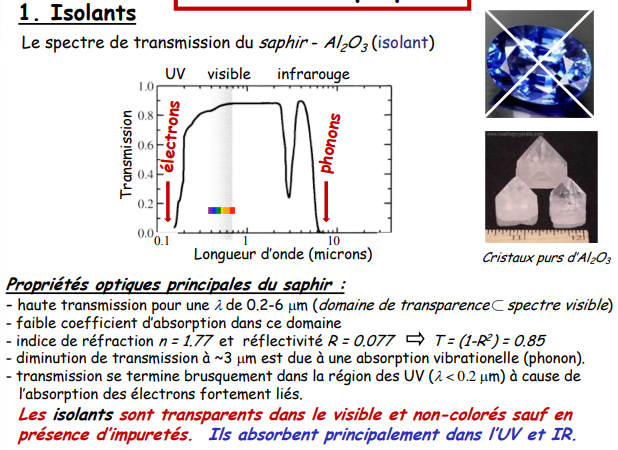
\includegraphics[width=0.75\linewidth]{Images/optique_isolant.png}
        \item \textbf{Semi-conducteurs} : Absorption sélective en fonction de la longueur d'onde. \\
            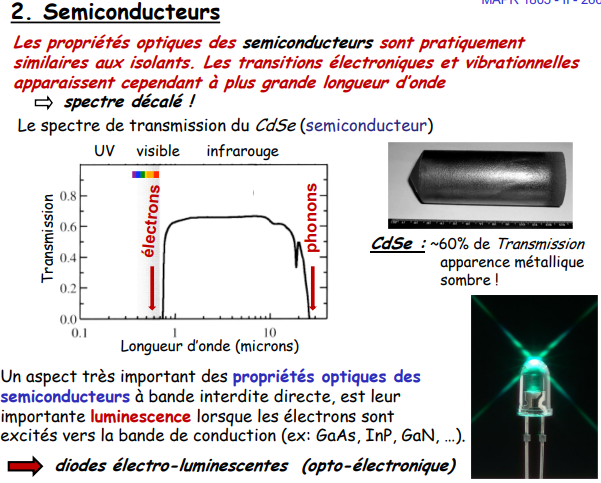
\includegraphics[width=0.75\linewidth]{Images/optique_semiconducteurs.png}
        \item \textbf{Verres} : Transparence dans le visible, fabriqués à partir de SiO$_2$ avec d'autres additifs. \\
            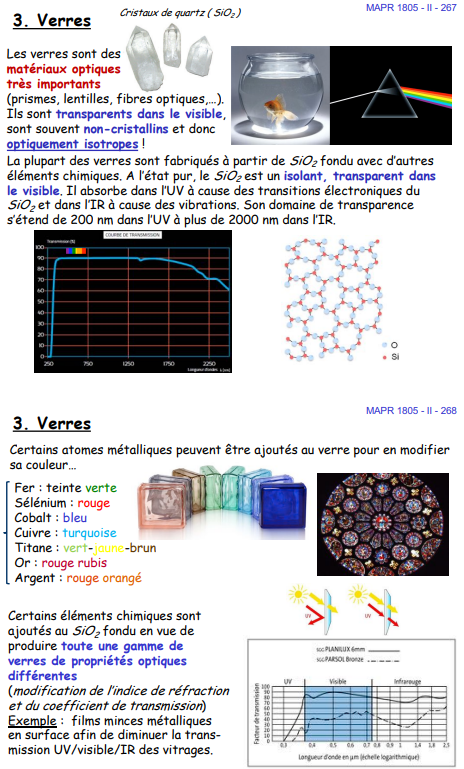
\includegraphics[width=0.75\linewidth]{Images/optique_verre.png}
        \item \textbf{Métaux} : Forte réflexion due aux électrons libres, absorbent dans l'UV. \\
            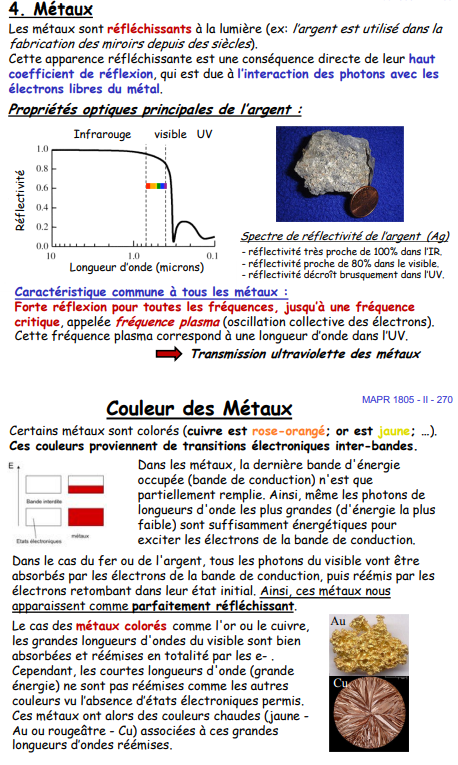
\includegraphics[width=0.75\linewidth]{Images/optique_metaux.png}
    \end{itemize}
    
    \subsection{Couleur des métaux et dopage des isolants}
    \begin{itemize}
        \item \textbf{Couleur des métaux} : Due aux transitions électroniques inter-bandes; les métaux colorés comme l'or et le cuivre présentent des couleurs chaudes.
        \item \textbf{Dopage des isolants} : Ajout d'impuretés pour modifier les propriétés optiques, comme dans le cas du rubis (saphir dopé au chrome).
    \end{itemize}
    
    \subsection{Fluorescence, phosphorescence, iridescence, diffraction, bioluminescence}
    \begin{itemize}
        \item \textbf{Fluorescence} : Émission rapide de lumière par un matériau après excitation.
        \item \textbf{Phosphorescence} : Émission prolongée de lumière après excitation, même après l'arrêt de la source lumineuse.
        \item \textbf{Iridescence} : Couleurs changeantes en raison d'interférences lumineuses.
        \item \textbf{Diffraction} : Déviation de la lumière autour d'obstacles ou à travers des ouvertures.
        \item \textbf{Bioluminescence} : Production de lumière par des organismes vivants via des réactions chimiques.
    \end{itemize}

\section{Déformation mécanique des solides}
    \subsection{Domaines de déformation}
    
    \begin{itemize}
        \item \textbf{Déformation du solide} : Résulte de l'application d'une force mécanique ou d'un déplacement, entraînant un changement de position des atomes ou molécules par rapport à leur position d'équilibre.
        \item \textbf{Domaines de déformation} :
        \begin{itemize}
            \item \textbf{Domaine élastique} : Les déformations sont réversibles et proportionnelles à la force appliquée. Pour la plupart des matériaux (sauf caoutchoucs), il s'agit de petites déformations.
            \item \textbf{Domaine plastique} : Les déformations sont irréversibles. Les grandes déformations sont caractéristiques de ce domaine.
        \end{itemize}
    \end{itemize}
    
    \subsection{Modes de déformation}
    
    \begin{itemize}
        \item Les matériaux peuvent être soumis à différents modes de chargement simples (homogènes) pour étudier leur réponse mécanique :
        \begin{itemize}
            \item \textbf{Extension / compression uniaxiale} : Application d'une force dans une seule direction, par exemple, une barre de traction.
            \item \textbf{Cisaillement (torsion) simple} : Exemple typique est un disque de frein.
            \item \textbf{Compression uniforme} : Forces identiques dans toutes les directions, comme pour un objet plongé dans l'eau.
        \end{itemize}
    \end{itemize}
    
    \subsection{Tenseur de déformation}
    
    \begin{itemize}
        \item Le tenseur de déformation décrit la déformation d'un matériau sous l'effet de contraintes appliquées. Il prend en compte les changements de longueur et d'angle dans les trois dimensions.
        \item \textbf{Composantes du tenseur de déformation} :
        \[
        \epsilon_{xx} = \frac{\Delta x}{x_0}, \quad \epsilon_{yy} = \frac{\Delta y}{y_0}, \quad \epsilon_{zz} = \frac{\Delta z}{z_0}
        \]
        \[
        \gamma_{xy} = \frac{\Delta x}{y_0}, \quad \gamma_{yz} = \frac{\Delta y}{z_0}, \quad \gamma_{zx} = \frac{\Delta z}{x_0}
        \]
    \end{itemize}
    
    \subsection{Essais mécaniques}
    
    \begin{itemize}
        \item Les essais mécaniques permettent de caractériser les propriétés mécaniques des matériaux. Ils incluent :
        \begin{itemize}
            \item \textbf{Essai de traction} : Mesure de la résistance d'un matériau à une force tirant en tension.
            \item \textbf{Essai de compression} : Mesure de la résistance d'un matériau à une force compressive.
            \item \textbf{Essai de torsion} : Évaluation de la résistance à une force de torsion appliquée.
            \item \textbf{Essai de flexion} : Détermination de la résistance d'un matériau lorsqu'il est soumis à une force qui cause une flexion.
            \item \textbf{Essai de fatigue} : Mesure de la capacité d'un matériau à résister à des charges cycliques.
            \item \textbf{Essai de fluage} : Détermination de la déformation lente d'un matériau sous une contrainte constante.
            \item \textbf{Essai de dureté} : Mesure de la résistance d'un matériau à la pénétration d'un objet dur.
        \end{itemize}
    \end{itemize}

\section{Propriétés mécaniques des différentes classes de matériaux}
    \subsection{La courbe de traction uniaxiale}
    
    \begin{itemize}
        \item \textbf{Courbe nominale} : Représente la contrainte nominale ($\sigma_E = F/S_0$) en fonction de la déformation nominale ($\epsilon_E = (L - L_0)/L_0$).
        \item \textbf{Module de Young} ($E$) : Correspond à la pente dans le régime élastique linéaire de la courbe de traction. Typiquement entre 50 et 300 GPa pour les métaux.
        \item \textbf{Limite d'élasticité} ($\sigma_0$) : Contrainte au-delà de laquelle la déformation plastique commence. Valeur typique entre 50 et 1000 MPa pour les métaux.
        \item \textbf{Allongement uniforme} ($A$) : Déformation à l'initiation de la striction. Peut atteindre 3 à 50\% pour les métaux.
        \item \textbf{Résistance mécanique} ($R_m$) : Contrainte maximale atteinte sur la courbe de traction. Valeur typique entre 100 et 1500 MPa.
        \item \textbf{Coefficient d'écrouissage} ($n$) : Indique la capacité du matériau à augmenter sa limite d'élasticité avec la déformation plastique.
    \end{itemize}
    
    \subsection{Propriétés mécaniques des matériaux}
    
    \begin{itemize}
        \item \textbf{Rigidité} : Capacité d'un matériau à résister à des déformations élastiques, mesurée par le module de Young ($E$).
        \item \textbf{Résistance} : Capacité à résister à l'entrée en plasticité, mesurée par la limite d'élasticité ($\sigma_0$).
        \item \textbf{Ductilité} : Capacité d'un matériau à subir des déformations plastiques avant rupture, mesurée par l'allongement à la rupture ($\epsilon_{nf}$) ou le coefficient de striction ($Z_f$).
        \item \textbf{Capacité d'écrouissage} : Indique l'évolution de la limite d'élasticité avec la déformation plastique, caractérisée par le coefficient d'écrouissage ($n$).
    \end{itemize}
    
    \subsection{Comportements indépendants du temps, de la vitesse de déformation et de la température}
    
    \begin{itemize}
        \item Les matériaux avec un comportement indépendant du temps, de la vitesse de déformation et de la température présentent des réponses mécaniques constantes dans ces conditions.
        \item \textbf{Matériaux élastiques linéaires} : Suivent la loi de Hooke, où $\sigma = E \epsilon$ avec $E$ constant.
        \item \textbf{Plasticité idéale} : La contrainte reste constante après le seuil de plasticité sans écrouissage.
    \end{itemize}
    
    \subsection{Comportements dépendants du temps, de la vitesse de déformation et de la température}
    
    \begin{itemize}
        \item Les matériaux avec un comportement dépendant du temps, de la vitesse de déformation et de la température présentent des réponses mécaniques qui varient avec ces paramètres.
        \item \textbf{Viscoélasticité} : Comportement intermédiaire entre les états solide élastique et fluide visqueux. La contrainte et la déformation varient avec le temps.
        \item \textbf{Relaxation de contrainte} : Décroissance de la contrainte avec le temps sous déformation constante.
        \item \textbf{Fluage} : Augmentation de la déformation avec le temps sous contrainte constante.
        \item \textbf{Température} : À des températures proches de la température de fusion ($T > 0.5 T_m$), les métaux et les céramiques peuvent montrer un comportement viscoélastique.
    \end{itemize}

\section{Aspects Thermodynamiques}
    \subsection{La dilatation thermique}
    
    \begin{itemize}
        \item \textbf{Dilatation thermique} : La dilatation thermique d'un matériau est sa tendance à changer de dimension en réponse à un changement de température.
        \item \textbf{Relation mathématique} : La déformation thermique ($\epsilon_{th}$) est proportionnelle à la variation de température ($\Delta T$) :
        \[
        \epsilon_{th} = \alpha \Delta T
        \]
        où $\alpha$ est le coefficient de dilatation thermique linéaire.
        \item \textbf{Origine physique} : La dilatation thermique est due à l'anharmonicité du potentiel d'interaction interatomique. Avec l'augmentation de la température, les atomes se déplacent de leurs positions d'équilibre, modifiant les distances interatomiques moyennes.
    \end{itemize}
    
    \subsection{Origine thermodynamique de la force de rétraction}
    
    \begin{itemize}
        \item \textbf{Force de rétraction} : Lorsqu'un matériau est déformé (par exemple, étendu uniaxialement), une force de rétraction ($F_r$) agit pour ramener le matériau à son état initial.
        \item \textbf{Variation de l'énergie interne} : La variation de l'énergie interne ($dU$) d'un système est donnée par :
        \[
        dU = T dS - p dV + F_r dL
        \]
        où $T$ est la température, $S$ l'entropie, $p$ la pression, $V$ le volume, et $L$ la longueur du matériau.
        \item \textbf{Origines de la force de rétraction} :
        \begin{itemize}
            \item \textbf{Composante enthalpique} : L'énergie mécanique est stockée sous forme d'augmentation de l'énergie interne, résultant de la mise sous tension des liaisons interatomiques.
            \item \textbf{Composante entropique} : L'énergie mécanique est dissipée sous forme de chaleur, augmentant l'entropie du système.
        \end{itemize}
        \item \textbf{Formule de la force de rétraction} :
        \[
        F_r = \left( \frac{\partial A}{\partial L} \right)_{V,T} = \left( \frac{\partial U}{\partial L} \right)_{V,T} - T \left( \frac{\partial S}{\partial L} \right)_{V,T}
        \]
        où $A$ est l'énergie libre de Helmholtz.
    \end{itemize}
    
    \subsection{Thermodynamique appliquée à la thermomécanique}
    
    \begin{itemize}
        \item \textbf{Équations thermodynamiques} : Les principes de la thermodynamique sont appliqués pour décrire les changements d'énergie et les forces internes dans les matériaux soumis à des contraintes thermiques et mécaniques.
        \item \textbf{Cas isotherme} : Pour des déformations à température constante ($dT = 0$) et faibles déformations, la variation de l'énergie libre de Helmholtz ($dA$) est donnée par :
        \[
        dA = F_r dL
        \]
        \item \textbf{Applications pratiques} : Ces concepts sont utilisés pour comprendre et prédire les comportements des matériaux sous des conditions de charge combinées thermiques et mécaniques, telles que le fluage et le vieillissement thermique des matériaux polymères et métalliques.
    \end{itemize}

\section{Défauts/microstructure/propriétés des matériaux métalliques et céramiques}
    \subsection{Origine physique de l’élasticité des matériaux enthalpiques}
    
    \begin{itemize}
        \item \textbf{Élasticité enthalpique} : L'élasticité d'un matériau est sa capacité à revenir à sa forme initiale après déformation. Pour les matériaux enthalpiques, l'élasticité est principalement due aux forces interatomiques résultant du potentiel interatomique.
        \item \textbf{Potentiel interatomique} : La force élastique provient de l'approximation harmonique du potentiel interatomique, comme décrit par le modèle de Lennard-Jones :
        \[
        U(r) = -U_{bond} \left[ 2 \left( \frac{r_0}{r} \right)^6 - \left( \frac{r_0}{r} \right)^{12} \right]
        \]
        où $U_{bond}$ est l'énergie de liaison et $r_0$ est la distance d'équilibre entre les atomes.
        \item \textbf{Module de Young} : Le module de Young ($E$) d'un matériau dépend de la raideur de la liaison chimique, de la densité du réseau cristallin ($N_v$), et de la distance interatomique :
        \[
        E = r_0^2 N_v \left( \frac{\partial^2 U}{\partial r^2} \right)_{r = r_0}
        \]
        \item \textbf{Exemples} : 
        \begin{itemize}
            \item Aluminium (CFC) : $E \approx 77.4 \, \text{GPa}$ avec une énergie de liaison $U_{bond} = 0.111 \, \text{eV}$.
            \item Fer (CC) : $E \approx 140 \, \text{GPa}$ avec $k_{bond} \approx 26.00 \, \text{N/m}$.
        \end{itemize}
    \end{itemize}
    
    \subsection{Origine physique de la résistance et de l’écrouissage des métaux}
    
    \begin{itemize}
        \item \textbf{Résistance des métaux} : La résistance mécanique des métaux est principalement déterminée par la limite d'élasticité ($\sigma_0$) et le coefficient d'écrouissage ($n$).
        \item \textbf{Mécanismes d'écrouissage} : L'écrouissage est le durcissement d'un métal par la déformation plastique. Il résulte de l'interaction et de la multiplication des dislocations dans le réseau cristallin.
        \item \textbf{Mécanismes de durcissement} : 
        \begin{itemize}
            \item \textbf{Forces de Peierls} : Résistance intrinsèque au mouvement des dislocations, fonction de la structure cristalline.
            \item \textbf{Écrouissage} : Augmentation de la densité de dislocations avec la déformation, suivant la loi de Taylor :
            \[
            \tau_w = G b \sqrt{\rho_d}
            \]
            où $G$ est le module de cisaillement, $b$ le vecteur de Burgers, et $\rho_d$ la densité de dislocations.
            \item \textbf{Durcissement par taille des grains} : Les joints de grains agissent comme des barrières au mouvement des dislocations, suivant la loi de Hall-Petch :
            \[
            \sigma_0 = \sigma_{osc} + k_g \frac{1}{\sqrt{d}}
            \]
            où $\sigma_{osc}$ est la limite d'élasticité du monocristal, $k_g$ le coefficient de Petch, et $d$ la taille moyenne des grains.
            \item \textbf{Durcissement par solution solide} : Les atomes en solution créent une distorsion du réseau qui augmente la résistance au mouvement des dislocations.
            \item \textbf{Durcissement par précipitation} : Interaction entre dislocations et précipités, contrôlée par la taille, la concentration, et la distribution des particules.
        \end{itemize}
    \end{itemize}

\section{Architecture moléculaire/microstructure/propriétés des matériaux polymères}
    \subsection{Élasticité caoutchoutique}
    
    \begin{itemize}
        \item \textbf{Élasticité caoutchoutique} : Comportement caractérisé par une réponse entropique à la déformation. Les chaînes polymères se réorganisent pour maximiser l'entropie.
        \item \textbf{Modèle de la chaîne libre (Freely Joint Chain, FJC)} : Modèle utilisé pour décrire le comportement d'un polymère, où la force de rétraction est proportionnelle à la température :
        \[
        F_r \approx 3k_BT \frac{r}{nb^2}
        \]
        où $k_B$ est la constante de Boltzmann, $T$ la température, $r$ la distance entre les extrémités de la chaîne, $n$ le nombre de segments, et $b$ la longueur des segments.
        \item \textbf{Force de rétraction entropique} : Augmente avec la température, résultat de la tendance des chaînes polymères à reprendre leur conformation initiale.
    \end{itemize}
    
    \subsection{Viscoélasticité des polymères}
    
    \begin{itemize}
        \item \textbf{Viscoélasticité} : Comportement intermédiaire entre les états solide élastique et fluide visqueux. La contrainte et la déformation varient avec le temps.
        \item \textbf{Relaxation de contrainte} : Décroissance de la contrainte sous déformation constante.
        \item \textbf{Fluage} : Augmentation de la déformation sous contrainte constante.
        \item \textbf{Module de relaxation} : Fonction du temps et de la température, mesurée par $E_r(t) = \frac{\sigma(t)}{\epsilon(t)}$.
    \end{itemize}
    
    \subsection{Module d’élasticité des polymères}
    
    \begin{itemize}
        \item \textbf{Module d'élasticité} : Dépend de la structure moléculaire et de la température. 
        \item \textbf{Régions caractéristiques} :
        \begin{itemize}
            \item \textit{Plateau vitreux} : Module élevé ($E > 1$ GPa) dû à l'élasticité enthalpique.
            \item \textit{Transition vitreuse} : Diminution rapide du module.
            \item \textit{Plateau caoutchoutique} : Module faible ($E \sim 1$ MPa) dû à l'élasticité entropique.
        \end{itemize}
    \end{itemize}
    
    \subsection{Comportement en traction des polymères}
    
    \begin{itemize}
        \item \textbf{Comportement en traction} : Dépend du type de polymère (amorphe, semi-cristallin).
        \item \textbf{Thermoplastiques ductiles} : Montrent un comportement élastique suivi d'un écrouissage, striction, et rupture.
        \item \textbf{Effet de la température} : Les polymères amorphes passent d'un comportement fragile à ductile avec l'augmentation de la température.
    \end{itemize}
    
    \subsection{Mécanismes de déformation plastique des polymères}
    
    \begin{itemize}
        \item \textbf{Déformation plastique} : Inclut la réorganisation des chaînes polymères et des lamelles cristallines.
        \item \textbf{Crazing (craquelure)} : Formation de micro-fissures sous contrainte, observable principalement dans les polymères amorphes.
        \item \textbf{Plasticité des lamelles cristallines} : Étapes de glissement, fragmentation et réorientation des lamelles.
    \end{itemize}
    
    \subsection{Les matériaux composites}
    
    \begin{itemize}
        \item \textbf{Matériaux composites} : Composés de deux ou plusieurs matériaux de natures différentes, combinant des propriétés complémentaires.
        \item \textbf{Types de fibres} : Fibres de carbone, fibres de verre, fibres de Kevlar.
        \item \textbf{Types de matrices} : Résines époxydes, polyesters, polymères haute performance.
        \item \textbf{Applications} : Utilisés pour leur légèreté et haute performance mécanique, par exemple dans l'aéronautique et l'automobile.
    \end{itemize}
\end{document}
